\documentclass{templateNote}
\usepackage{soul}
\usepackage{overpic}
\begin{document}

\imagenlogoU{img/LogoElNube.png}
\linklogoU{https://github.com/MarceloPazPezo}
\imagenlogoD{img/LogoNGM.png}
\linklogoD{https://github.com/NicoGomezM}
\linkQRDoc{https://github.com/MarceloPazPezo/MyRepo/blob/main/Icinf/Semestre\%207/Sistemas\%20de\%20Informaci\%C3\%B3n/Test\%202/Test-2.pdf}
\titulo{Test 2}
\asignatura{Sistemas de Informaci\'on}
\autor{
Marcelo Paz\\
Nicol\'as G\'omez\\
Javier Santander
}
\vDoc{1.0.1}

% Metadatos del PDF
\title{[\asignatura]-\titulo}
\author{
    \autor
}
\portada
\margenes % Crear márgenes
\section{Recordatorio}
\textbf{Representación de un sistema}
\begin{center}
    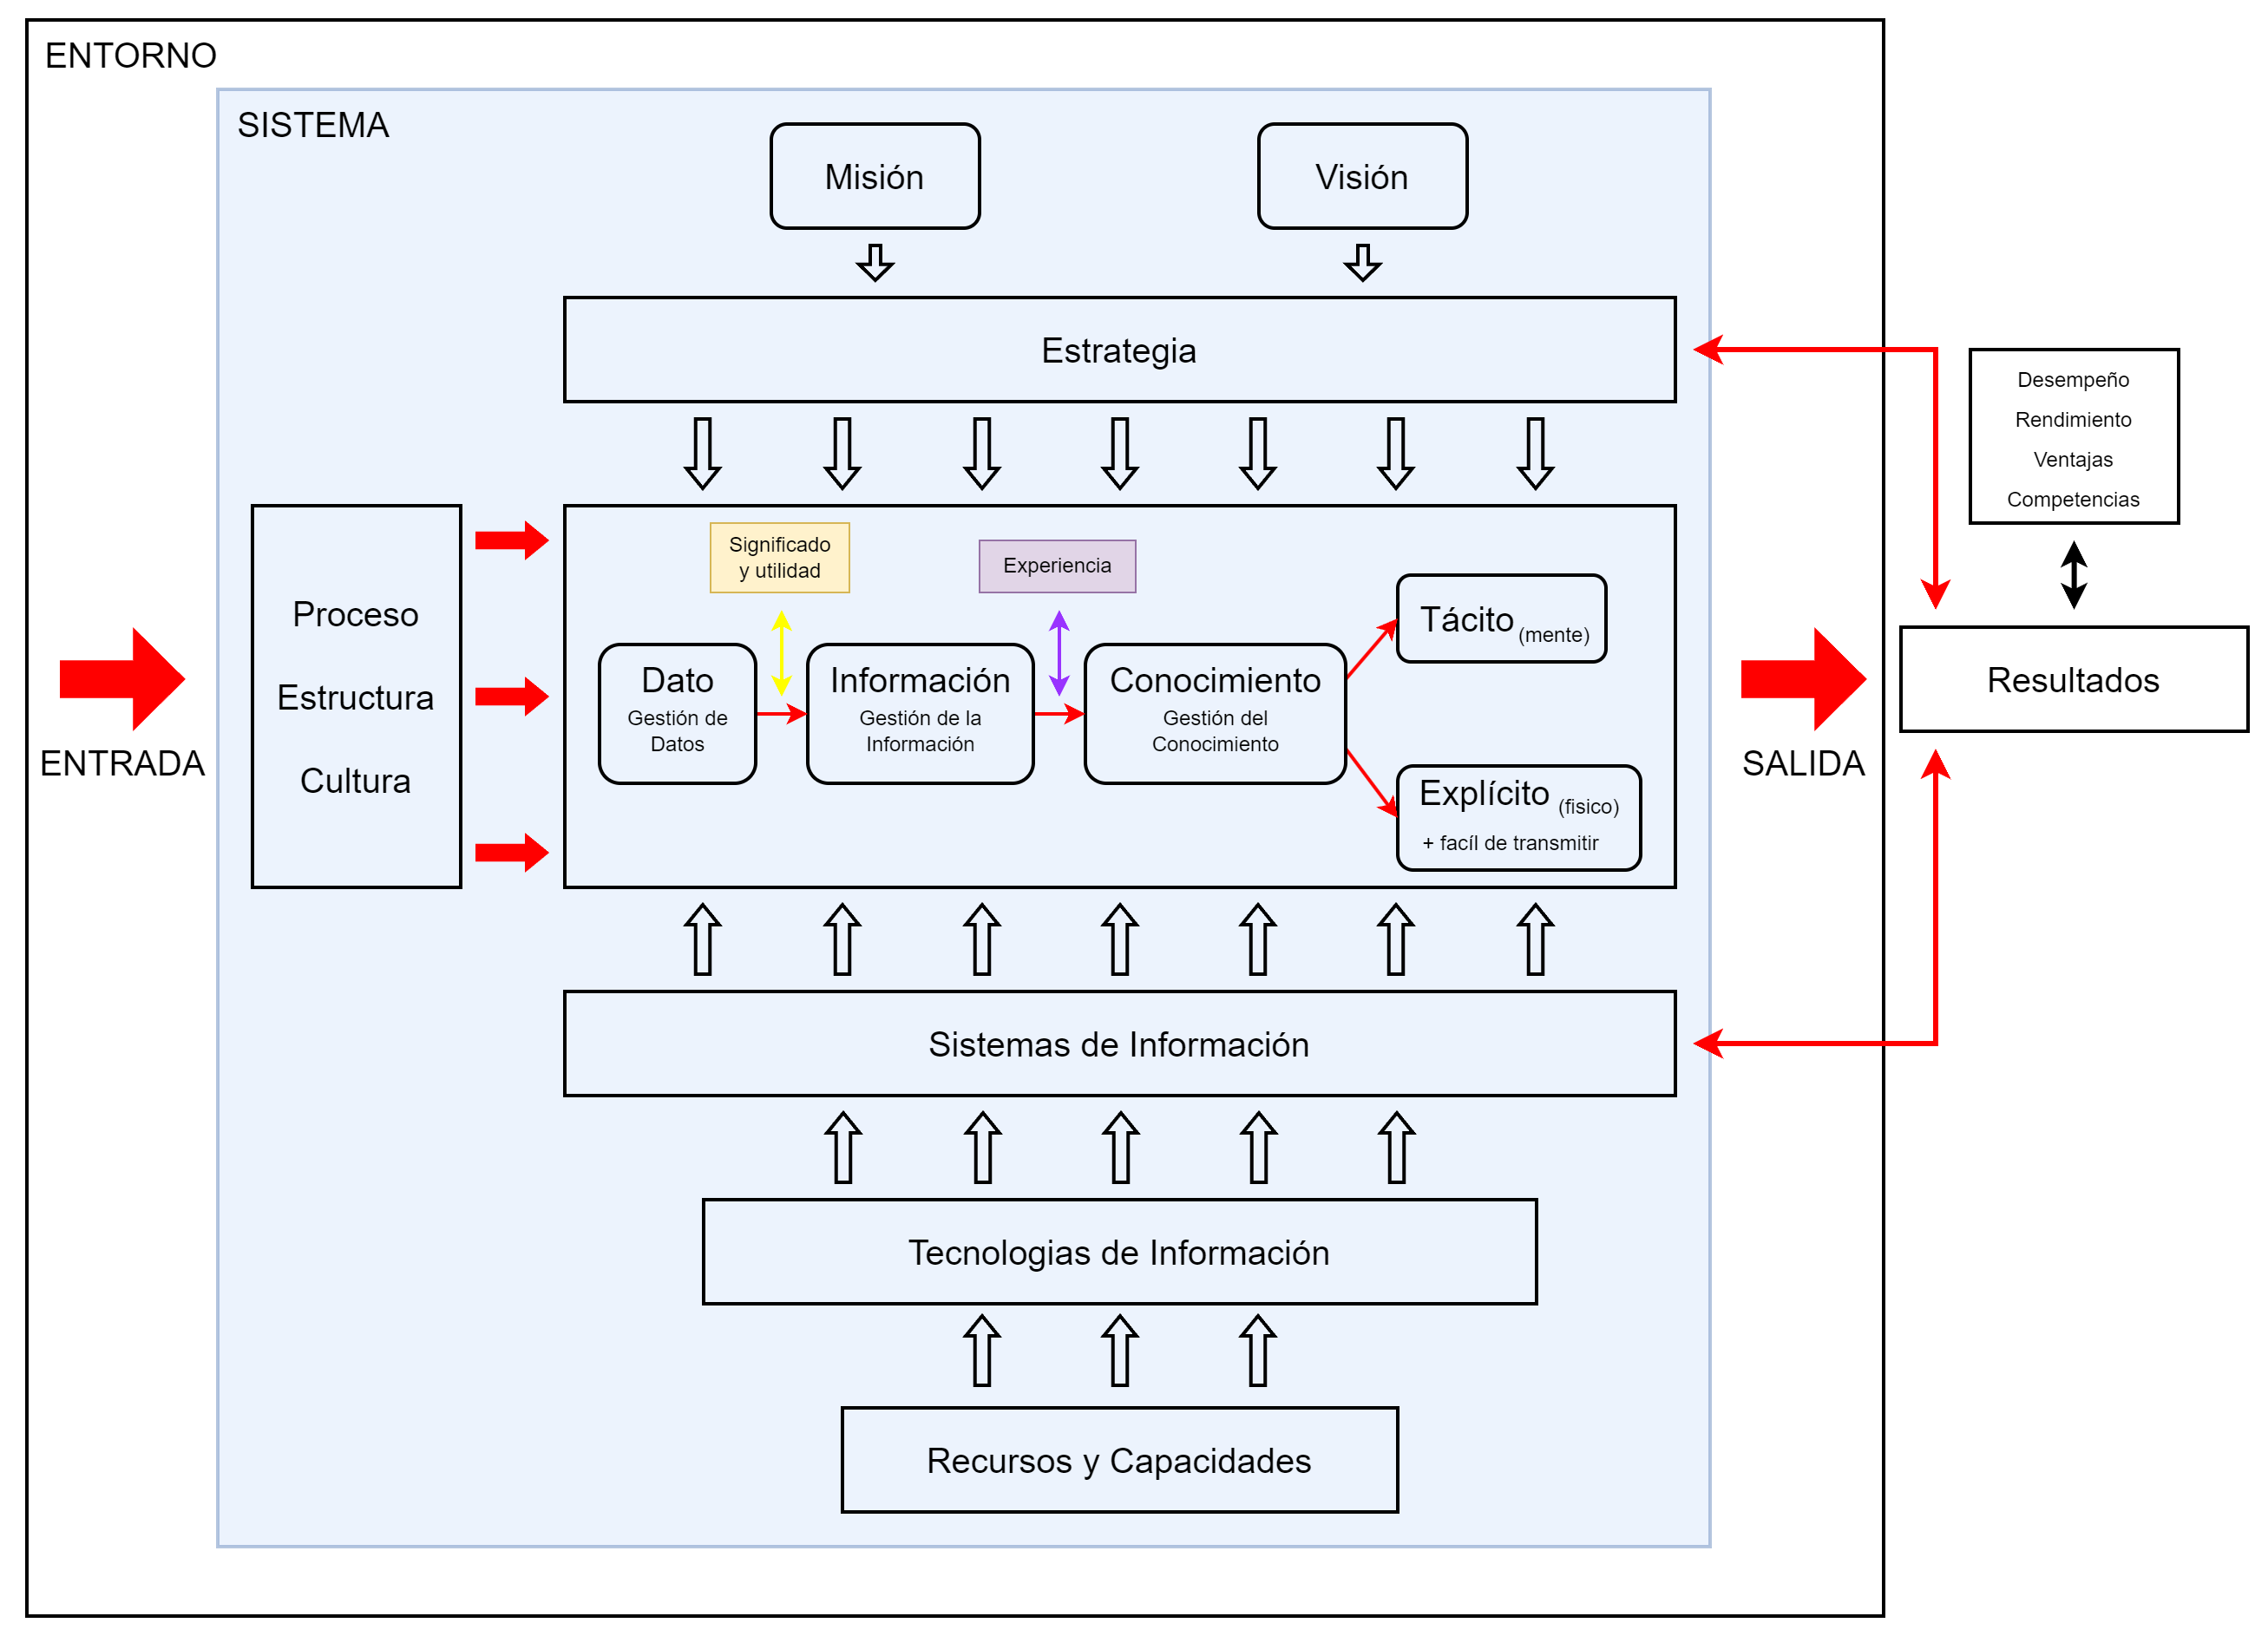
\includegraphics[width=0.8\textwidth]{img/digramaCompleto.png}
\end{center}
\noindent
\textbf{S.I.:} \hl{Conjunto formal de procesos} que operando sobre una \hl{colección de datos estructurados} recopila, elabora y distribuye (parte de) la información \hl{necesaria para la operación de dicha empresa} y para las actividades de \hl{dirección y control} correspondientes apoyando al menos en parte la toma de \hl{decisiones necesarias} para desempeñar las \hl{funciones y procesos} de acuerdo con la \hl{estrategia.}
\begin{itemize}
    \item Un proceso es formal cuando esta bien definido, este proceso se puede estudiar.
    \item Un proceso es informal cuando no esta bien definido.
    \item Los datos estan estructurados según la necesidad de la empresa.
    \item Recopilación, elaboración y distribución $\rightarrow$ Sistema con entrada, proceso y salida.
\end{itemize}

\newpage
\textbf{Piramide de Anthony.}
\begin{center}
    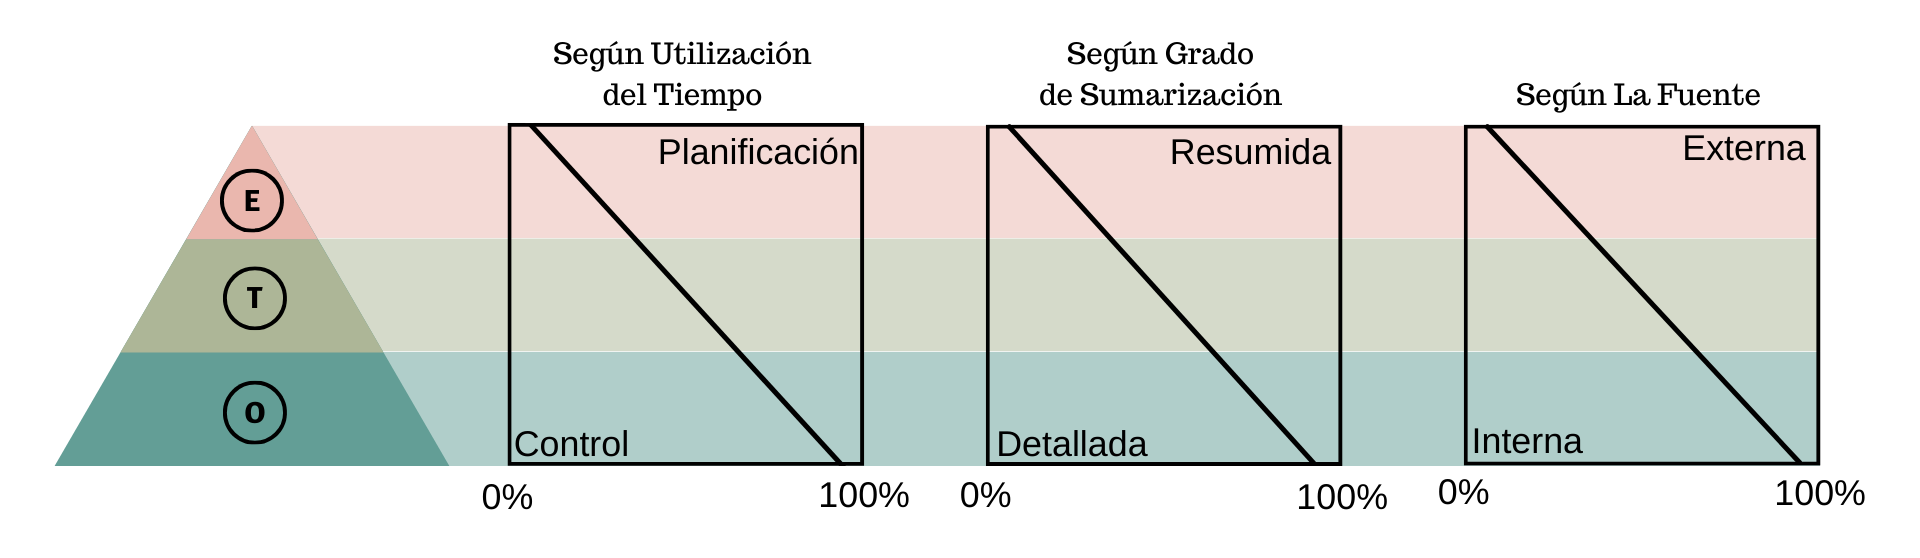
\includegraphics[width=\textwidth]{img/PiramideAnthony2.png}
\end{center}

\textbf{Curva de Nolan.}
\begin{center}
    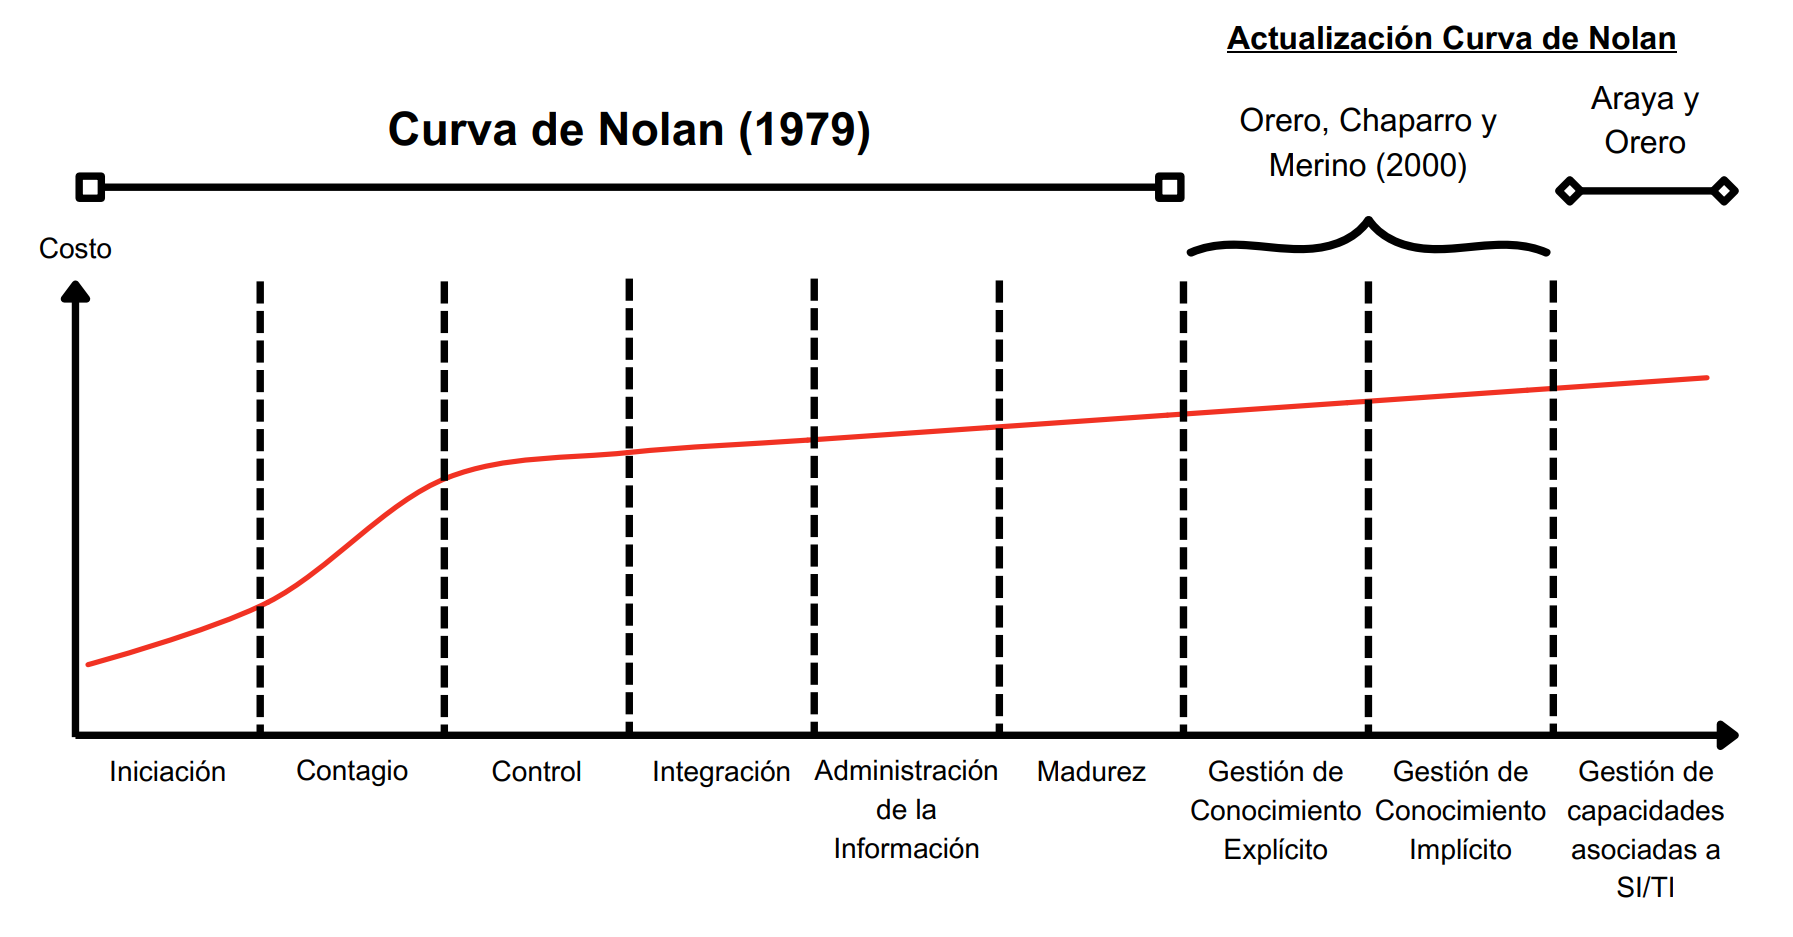
\includegraphics[width=\textwidth]{img/CurvaDeNolanActualizada.png}
\end{center}


\section{Transformación digital}
Implementación de las tecnologías digitales en las empresas para cambiar la forma en que se hacen las cosas.\newline
\textbf{Características:}
\begin{itemize}
    \item Mejora la productividad.
    \item Mejora la experiencia del cliente.
    \item Reduce los costos operativos.
\end{itemize}
\textbf{Desventajas:}
\begin{itemize}
    \item Alto nivel de competitividad.
    \item Necesidad de una evolución constante en la industria.
    \item Impacto en el ámbito cultural de las personas.
\end{itemize}

\section{Reingeniería de procesos}
\noindent Rediseño radical de procesos para lograr mejoras significativas en medidas críticas y contemporáneas de rendimiento, como costos, calidad, servicio y rapidez.
\begin{itemize}
    \item \textbf{Objetivos:}
    \begin{itemize}
        \item Reducción de costos.
        \item Mejora de la calidad.
        \item Reducción de tiempos.
        \item Mejora de la satisfacción del cliente.
    \end{itemize}
    \item \textbf{Características:}
    \begin{itemize}
        \item Cambio radical.
        \item Enfocado en procesos.
        \item Mejora de la eficiencia.
        \item Mejora de la eficacia.
        \item Mejora de la calidad.
        \item Mejora de la satisfacción del cliente.
        \item Rapidez, obteniendo resultados en corto plazo.
    \end{itemize}
    \item \textbf{Desventajas:}
    \begin{itemize}
        \item Resistencia al cambio.
        \item Es de alto riesgo.
        \item Despidos debido a la toma de este riesgo.
    \end{itemize}
\end{itemize}

\section{Industria 4.0}
\noindent Es la cuarta revolución industrial, se caracteriza por la digitalización de la industria. Se basa en la interconexión de sistemas ciber-físicos, la inteligencia artificial, la robótica, el big data, la computación en la nube, la realidad aumentada, la impresión 3D, la ciberseguridad, la internet de las cosas, la simulación y la integración de sistemas.
\begin{itemize}
    \item \textbf{Características:}
    \begin{itemize}
        \item Productor tiene conciencia del cambio en su forma de trabajar y el cliente mejora el producto final.
        \item Aumento en la seguridad de los trabajadores.
        \item Mejora toma decisiones (Bases digitales).
        \item Aumento de competitividad.
    \end{itemize}

    \newpage
    \item \textbf{Riesgos:}
    \begin{itemize}
        \item Dependencia tecnológica (Brecha digital).
        \item Posibilidad de ataques cibernéticos.
        \item Aumento despidos y contrataciones selectivas.
        \item Resistencia al cambio.
    \end{itemize}
\end{itemize}
\section{Internet de las cosas (IOT)}
\noindent El IOT es una herramienta que permite la interconexión de objetos cotidianos a la red, permitiendo la comunicación entre ellos y la recolección de datos. Esta herramienta se aplica a la vida cotidiana y a la industria.

\begin{itemize}
    \item \textbf{Características:}
    \begin{itemize}
        \item Conectividad con la red.
        \item Sensibilidad en parámetros analizables.
        \item Interacción entre elementos a través de interfaces para el usuario.
        \item Nivel de seguridad.
        \item Automatización de tareas y optimización de procesos industriales.
    \end{itemize}
    \item \textbf{Ventajas:}
    \begin{itemize}
        \item Mejora la eficiencia.
        \item Mejora la calidad de vida.
        \item Mayor facilidad en el seguimiento de procesos para las empresas.
        \item Optimización de tiempos.
    \end{itemize}
    \item \textbf{Desventajas:}
    \begin{itemize}
        \item Vulnerabilidad en la seguridad.
        \item Costos de implementación.
        \item Dependencia de la tecnología (Brecha digital).
        \item Resistencia cultural por parte del usuario.
    \end{itemize}
\end{itemize}
\newpage
\section{Paradoja de la productividad}
\noindent
\textbf{Palabras claves:}
\begin{itemize}
    \item S.I. : Herramienta para manejar los datos de informaci\'on de cualquier empresa.
    \item T.I. : Herramientas que pueden almacenar y transmitir informaci\'on de manera digital.
\end{itemize}

\noindent
\textbf{Resumen:}

La paradoja de la productividad en los sistemas de informaci\'on, surgio entre los 70 y 80, se refiere a la disminuci\'on de la productividad de los sistemas de informaci\'on, a pesar de que se esperaba que aumentara.\\
\textbf{Comentarios:}
\begin{itemize}
    \item Pensaron que por el solo hecho de tener T.I. subir\'ia la productividad.
    \item Tenian muchos T.I. pero no las capacidades para usarlas.
    \item La principal causa del fracaso de un S.I. son las personas.
    \item Esto se repite en la historia.
\end{itemize}
\begin{center}
    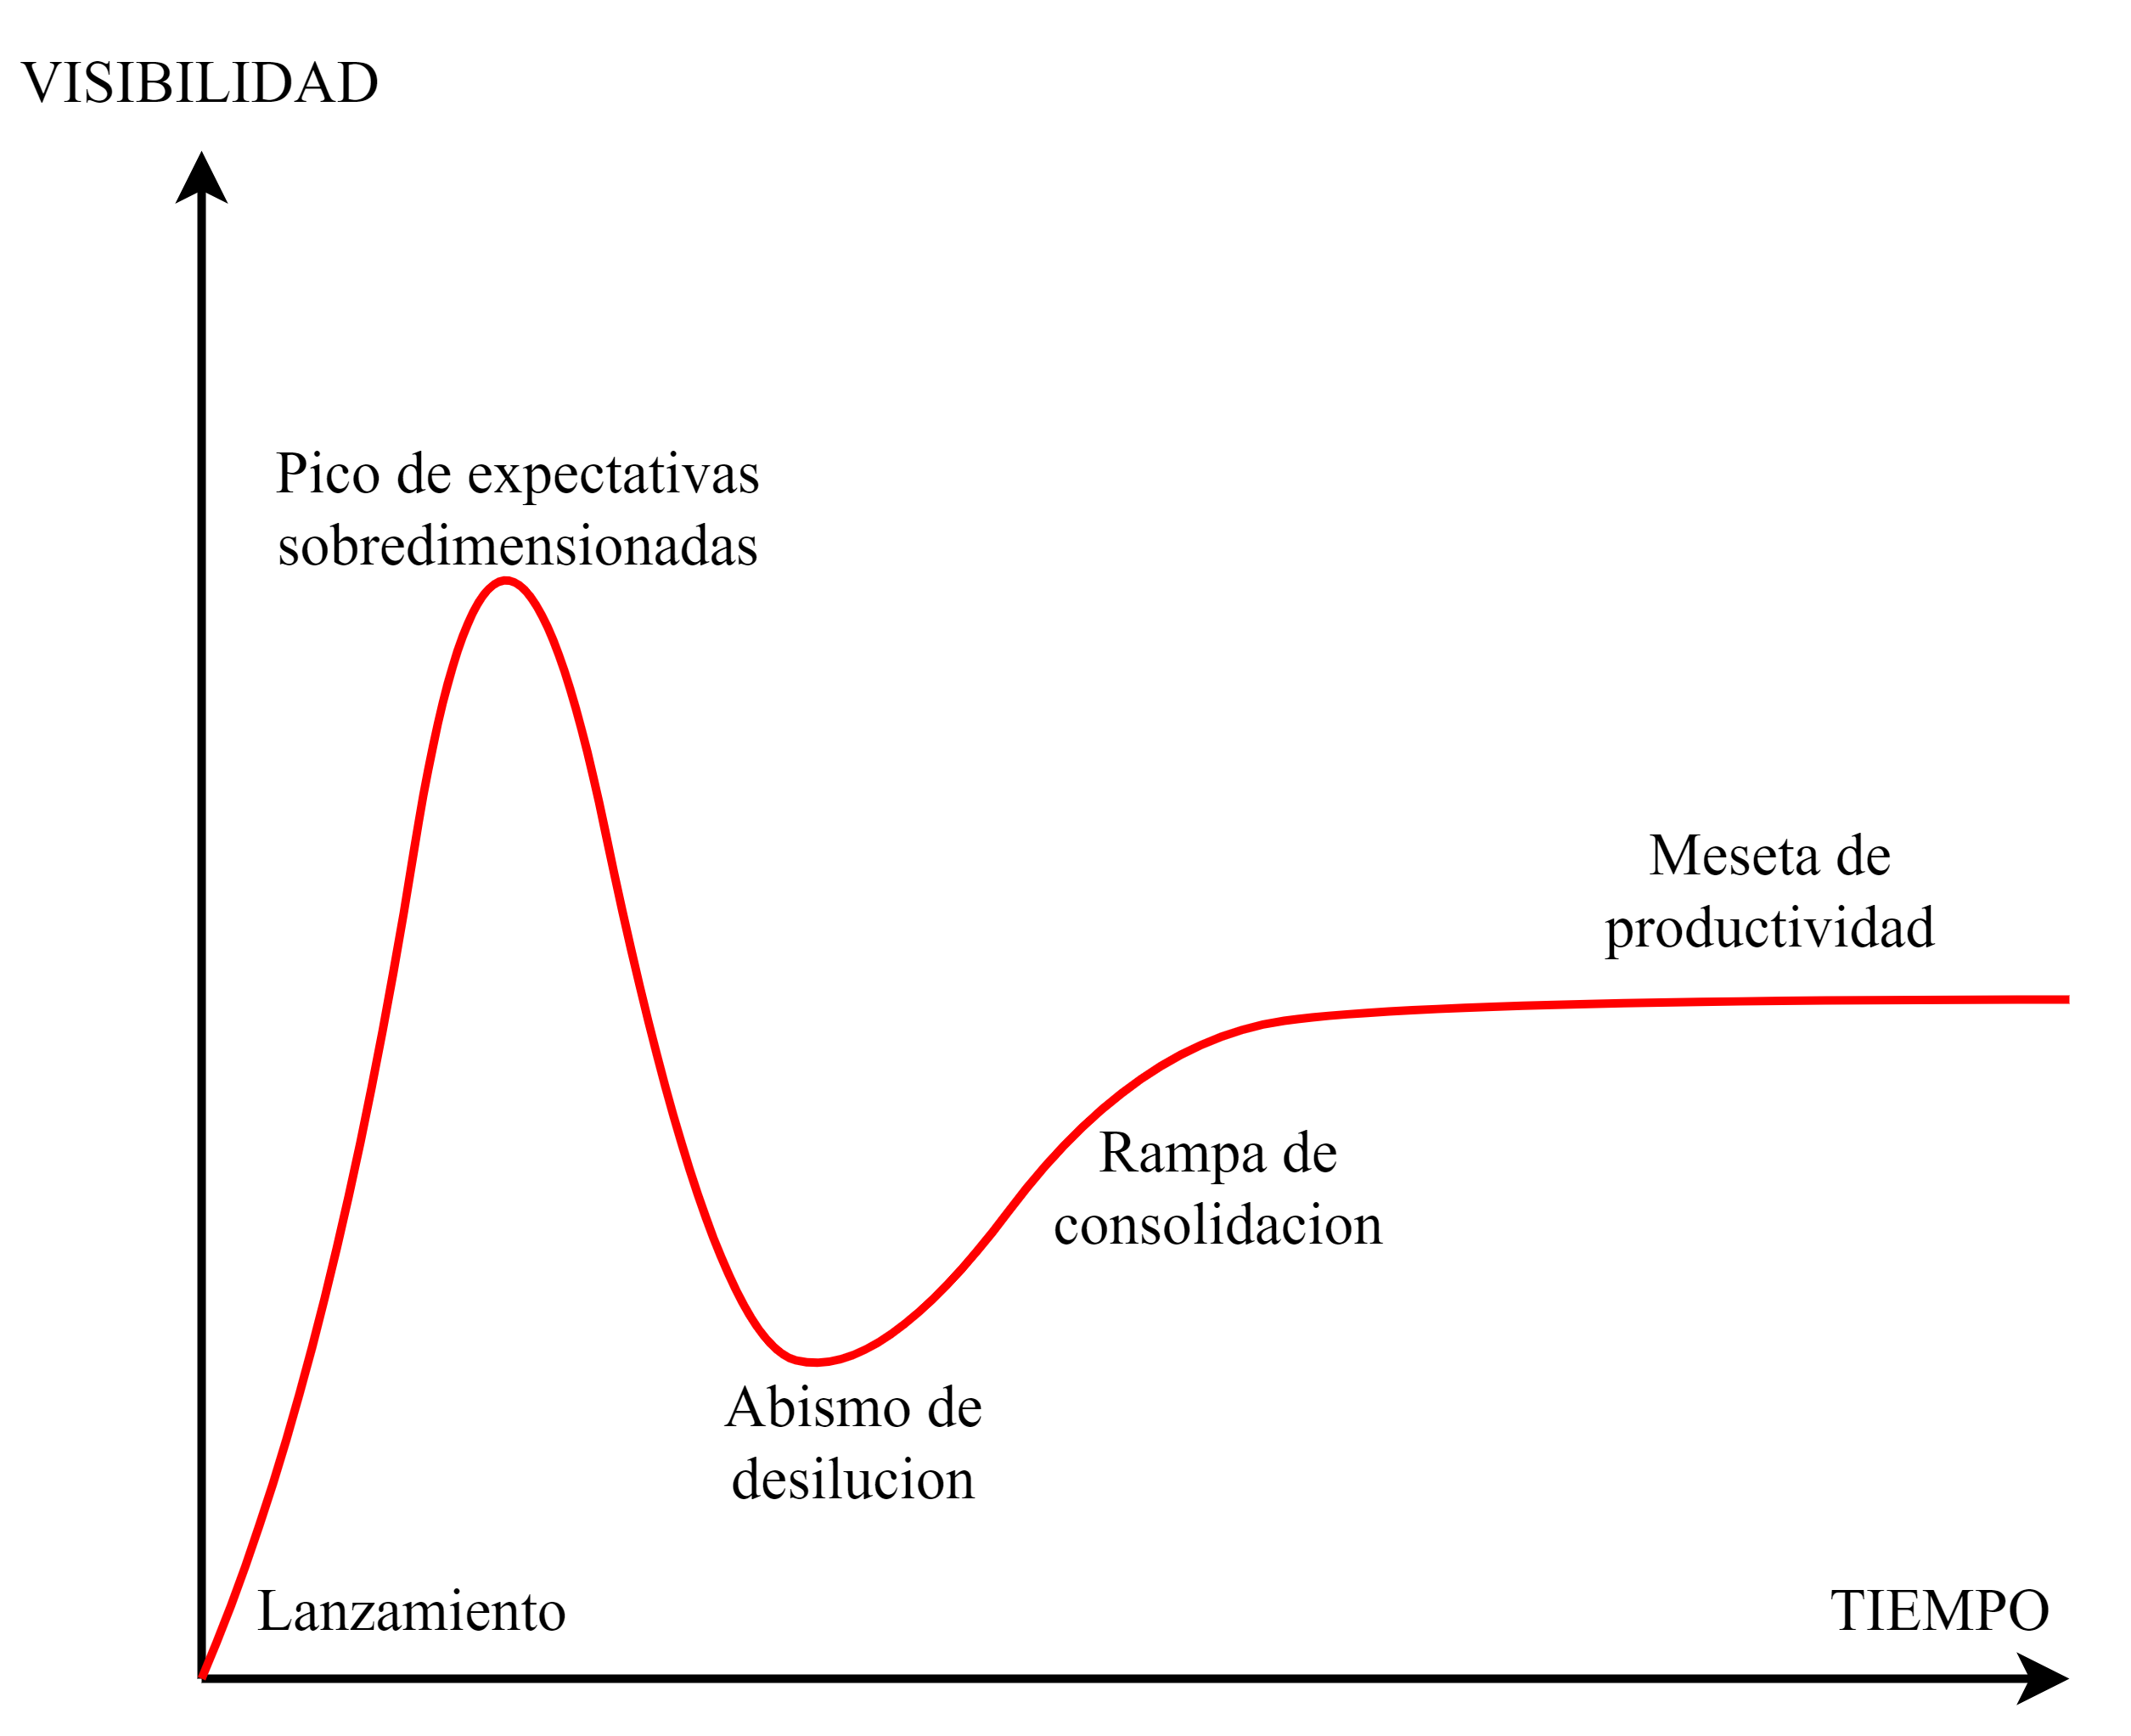
\includegraphics[width=0.7\textwidth]{diagram/ParadojaProductividad.png}
\end{center}
Etapas de la curva:
\begin{itemize}
    \item Lanzamiento: Se lanza un nuevo producto y se espera que la productividad aumente.
    \item Pico de expectativas sobredimensionadas: Se espera que la productividad aumente, pero no lo hace.
    \item Abismo de desilusi\'on: La productividad disminuye.
    \item Rampa de la consolidaci\'on: La productividad aumenta.
    \item Meseta de la productividad: La productividad se mantiene.
\end{itemize}

\newpage
\subsection{An\'alisis de la gr\'afica}
Cuando un empresa incorpora algun S.I. la gr\'afica productividad v/s tiempo tiende a parecerse a lo siguiente:
\begin{center}
    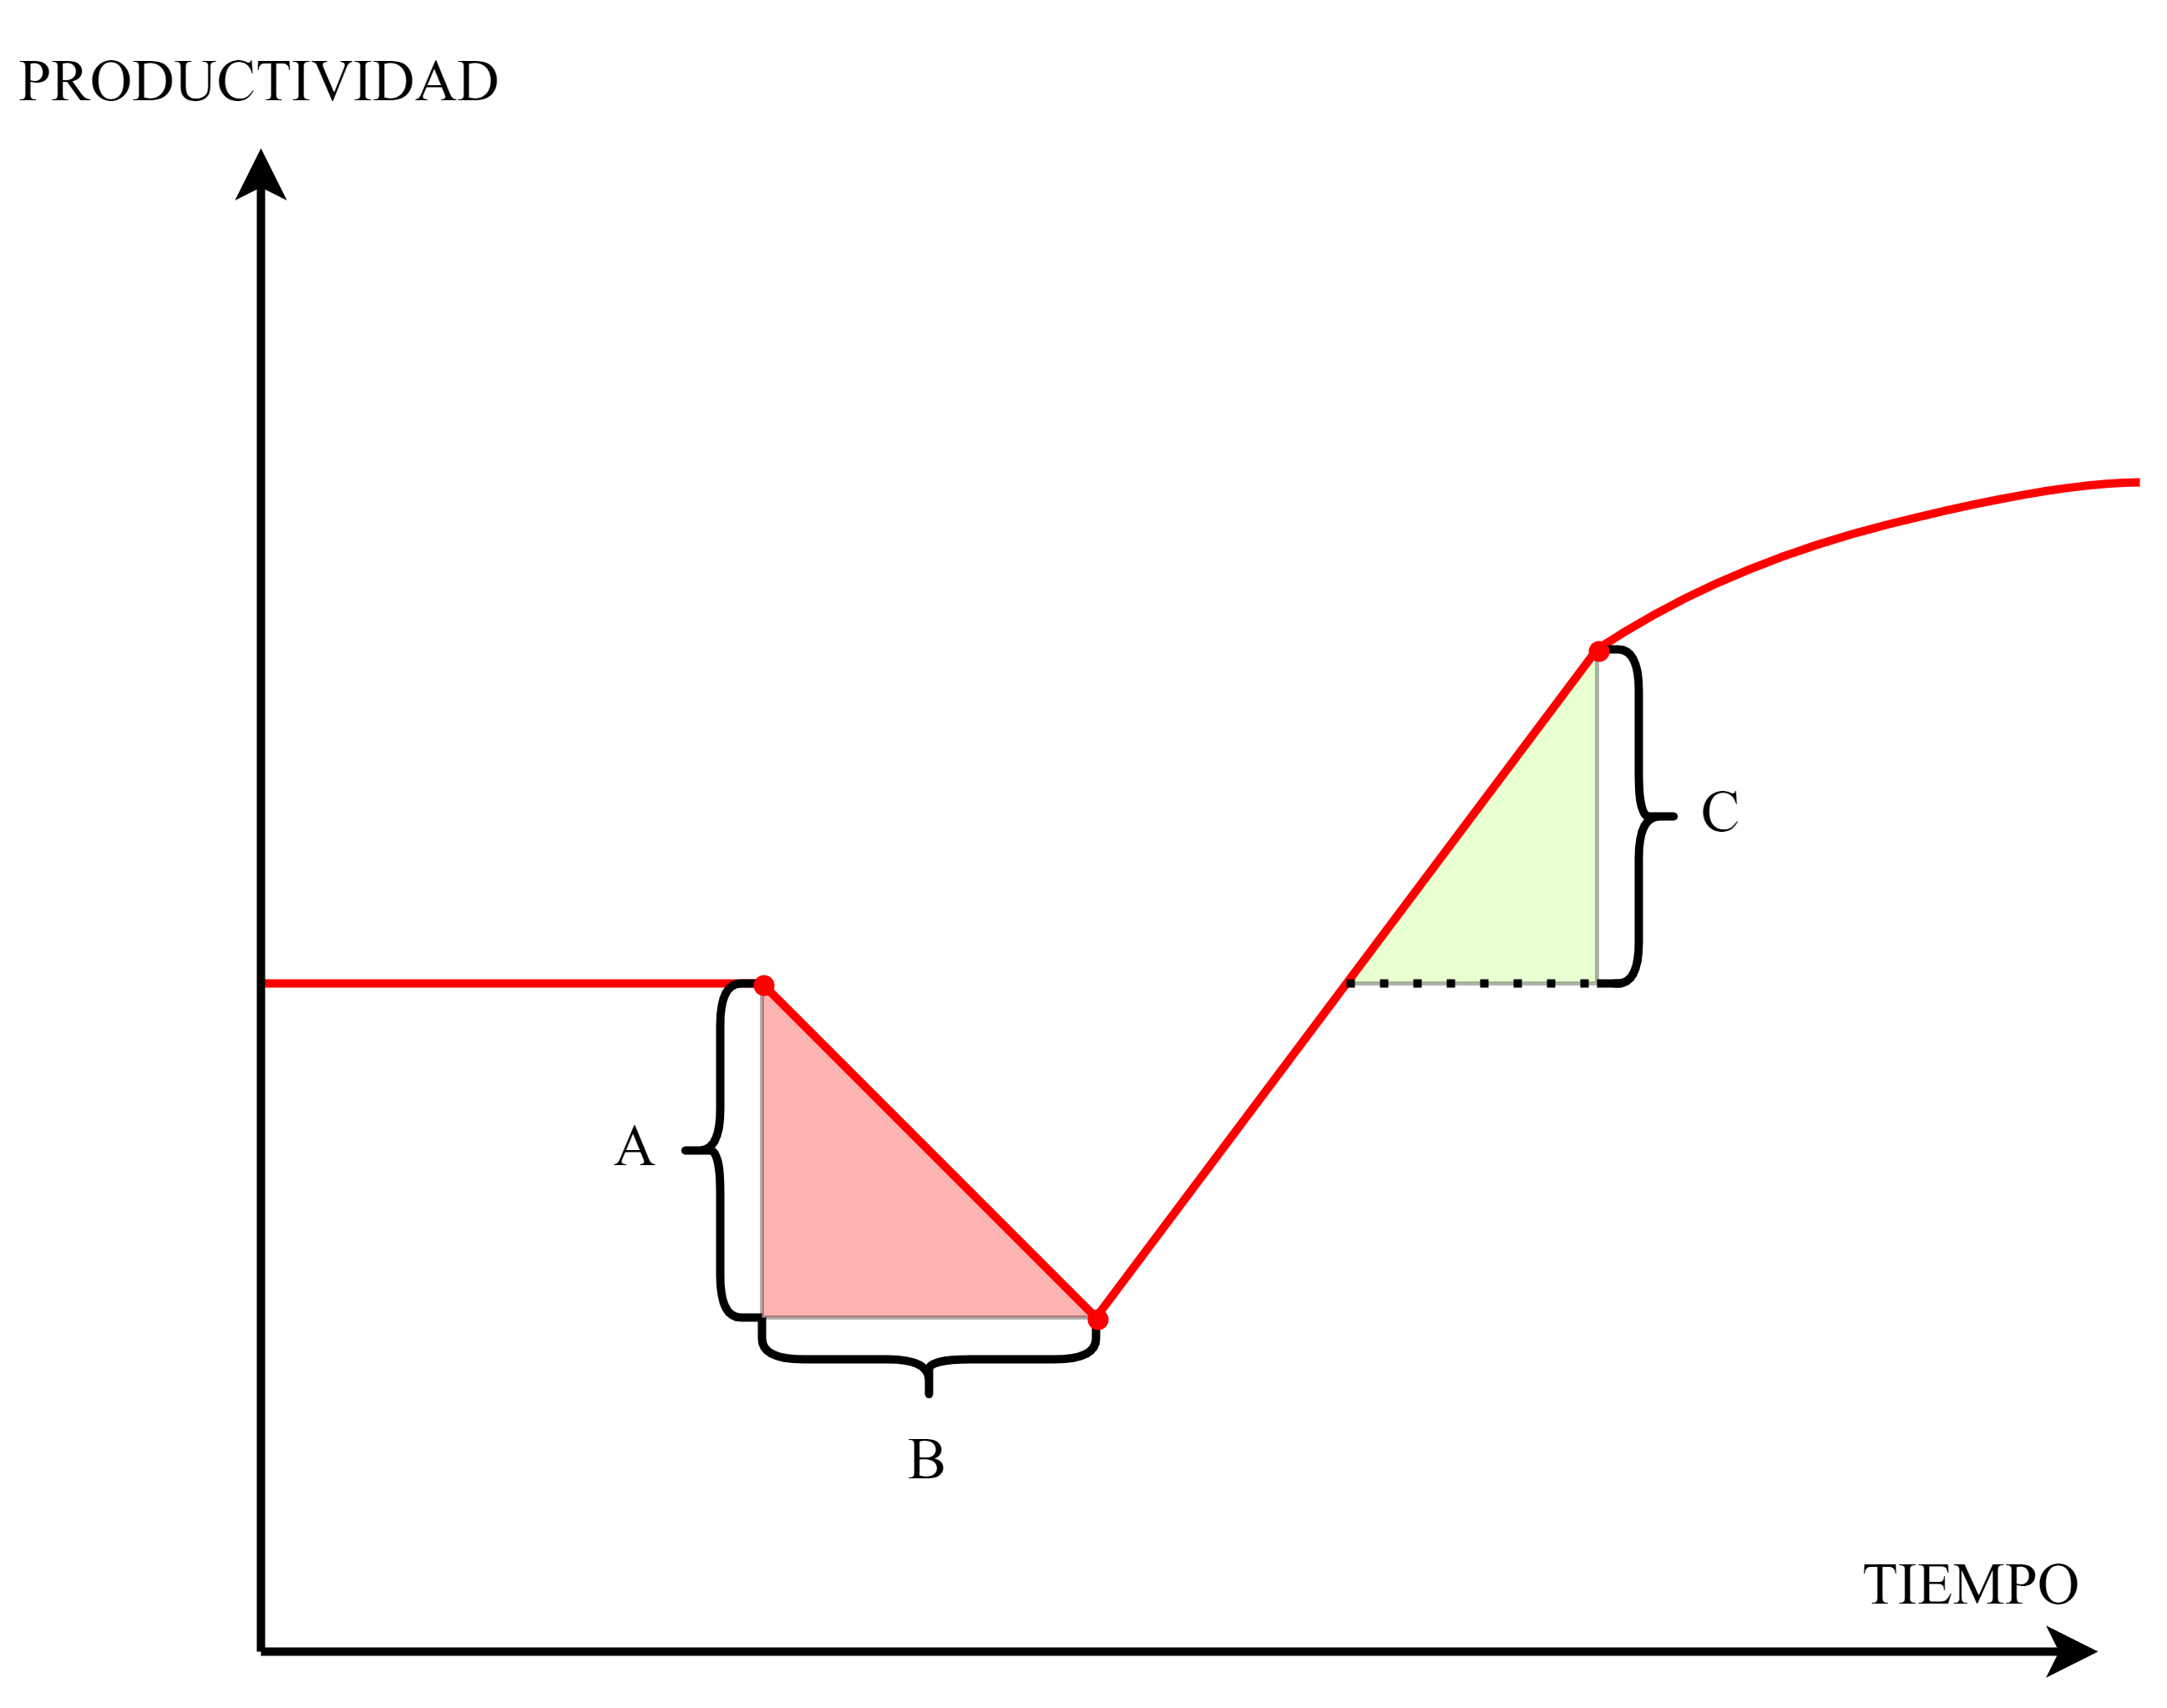
\includegraphics[width=0.7\textwidth]{diagram/AnalisisProductividad.png}
\end{center}

Podemos observar que \hl{baja la productividad} en A unidades por un tiempo B, esto ocurre \hl{por la resistencia al cambio de la gente} (cultura).
Luego en alg\'un momento la gente aprendera a usar el S.I y el T.I, aumentando la productividad.
Al final en algun punto se superara la productividad anterior al S.I. aumentando C unidades.

Tras este peque\~no an\'alisis, nuestro objetivo es disminuir A y B con 3 formas:
\begin{enumerate}
    \item \textbf{Facilitaci\'on de participaci\'on:} Hacer que la gente/usuarios participen del proceso de cambio.
    \item \textbf{Facilitaci\'on de aprendizaje:} Hacer capacitaciones.
    \item \textbf{Asistencia a usuarios:} Soporte.
\end{enumerate}

\newpage
\section{Proceso de Desarrollo de un S.I.}
\subsection{Etapas}
\begin{enumerate}
    \item \textbf{Concepci\'on (Fuente de solicitud):} Un S.I. surge del pensamiento de alguien al ver/tener una necesidad.
    \item \textbf{Dise\~no:} Se utilizan procesos, estrategias y tecnicas de modelado para cumplir con los requierimientos.
    \item \textbf{Construcci\'on:} Se construye el S.I. seg\'un el dise\~no.
    \item \textbf{Implementaci\'on:} Se pone en marcha el S.I.
\end{enumerate}

\subsubsection{Concepci\'on:}
\subsubsection*{Fuentes de solicitud}
\begin{center}
    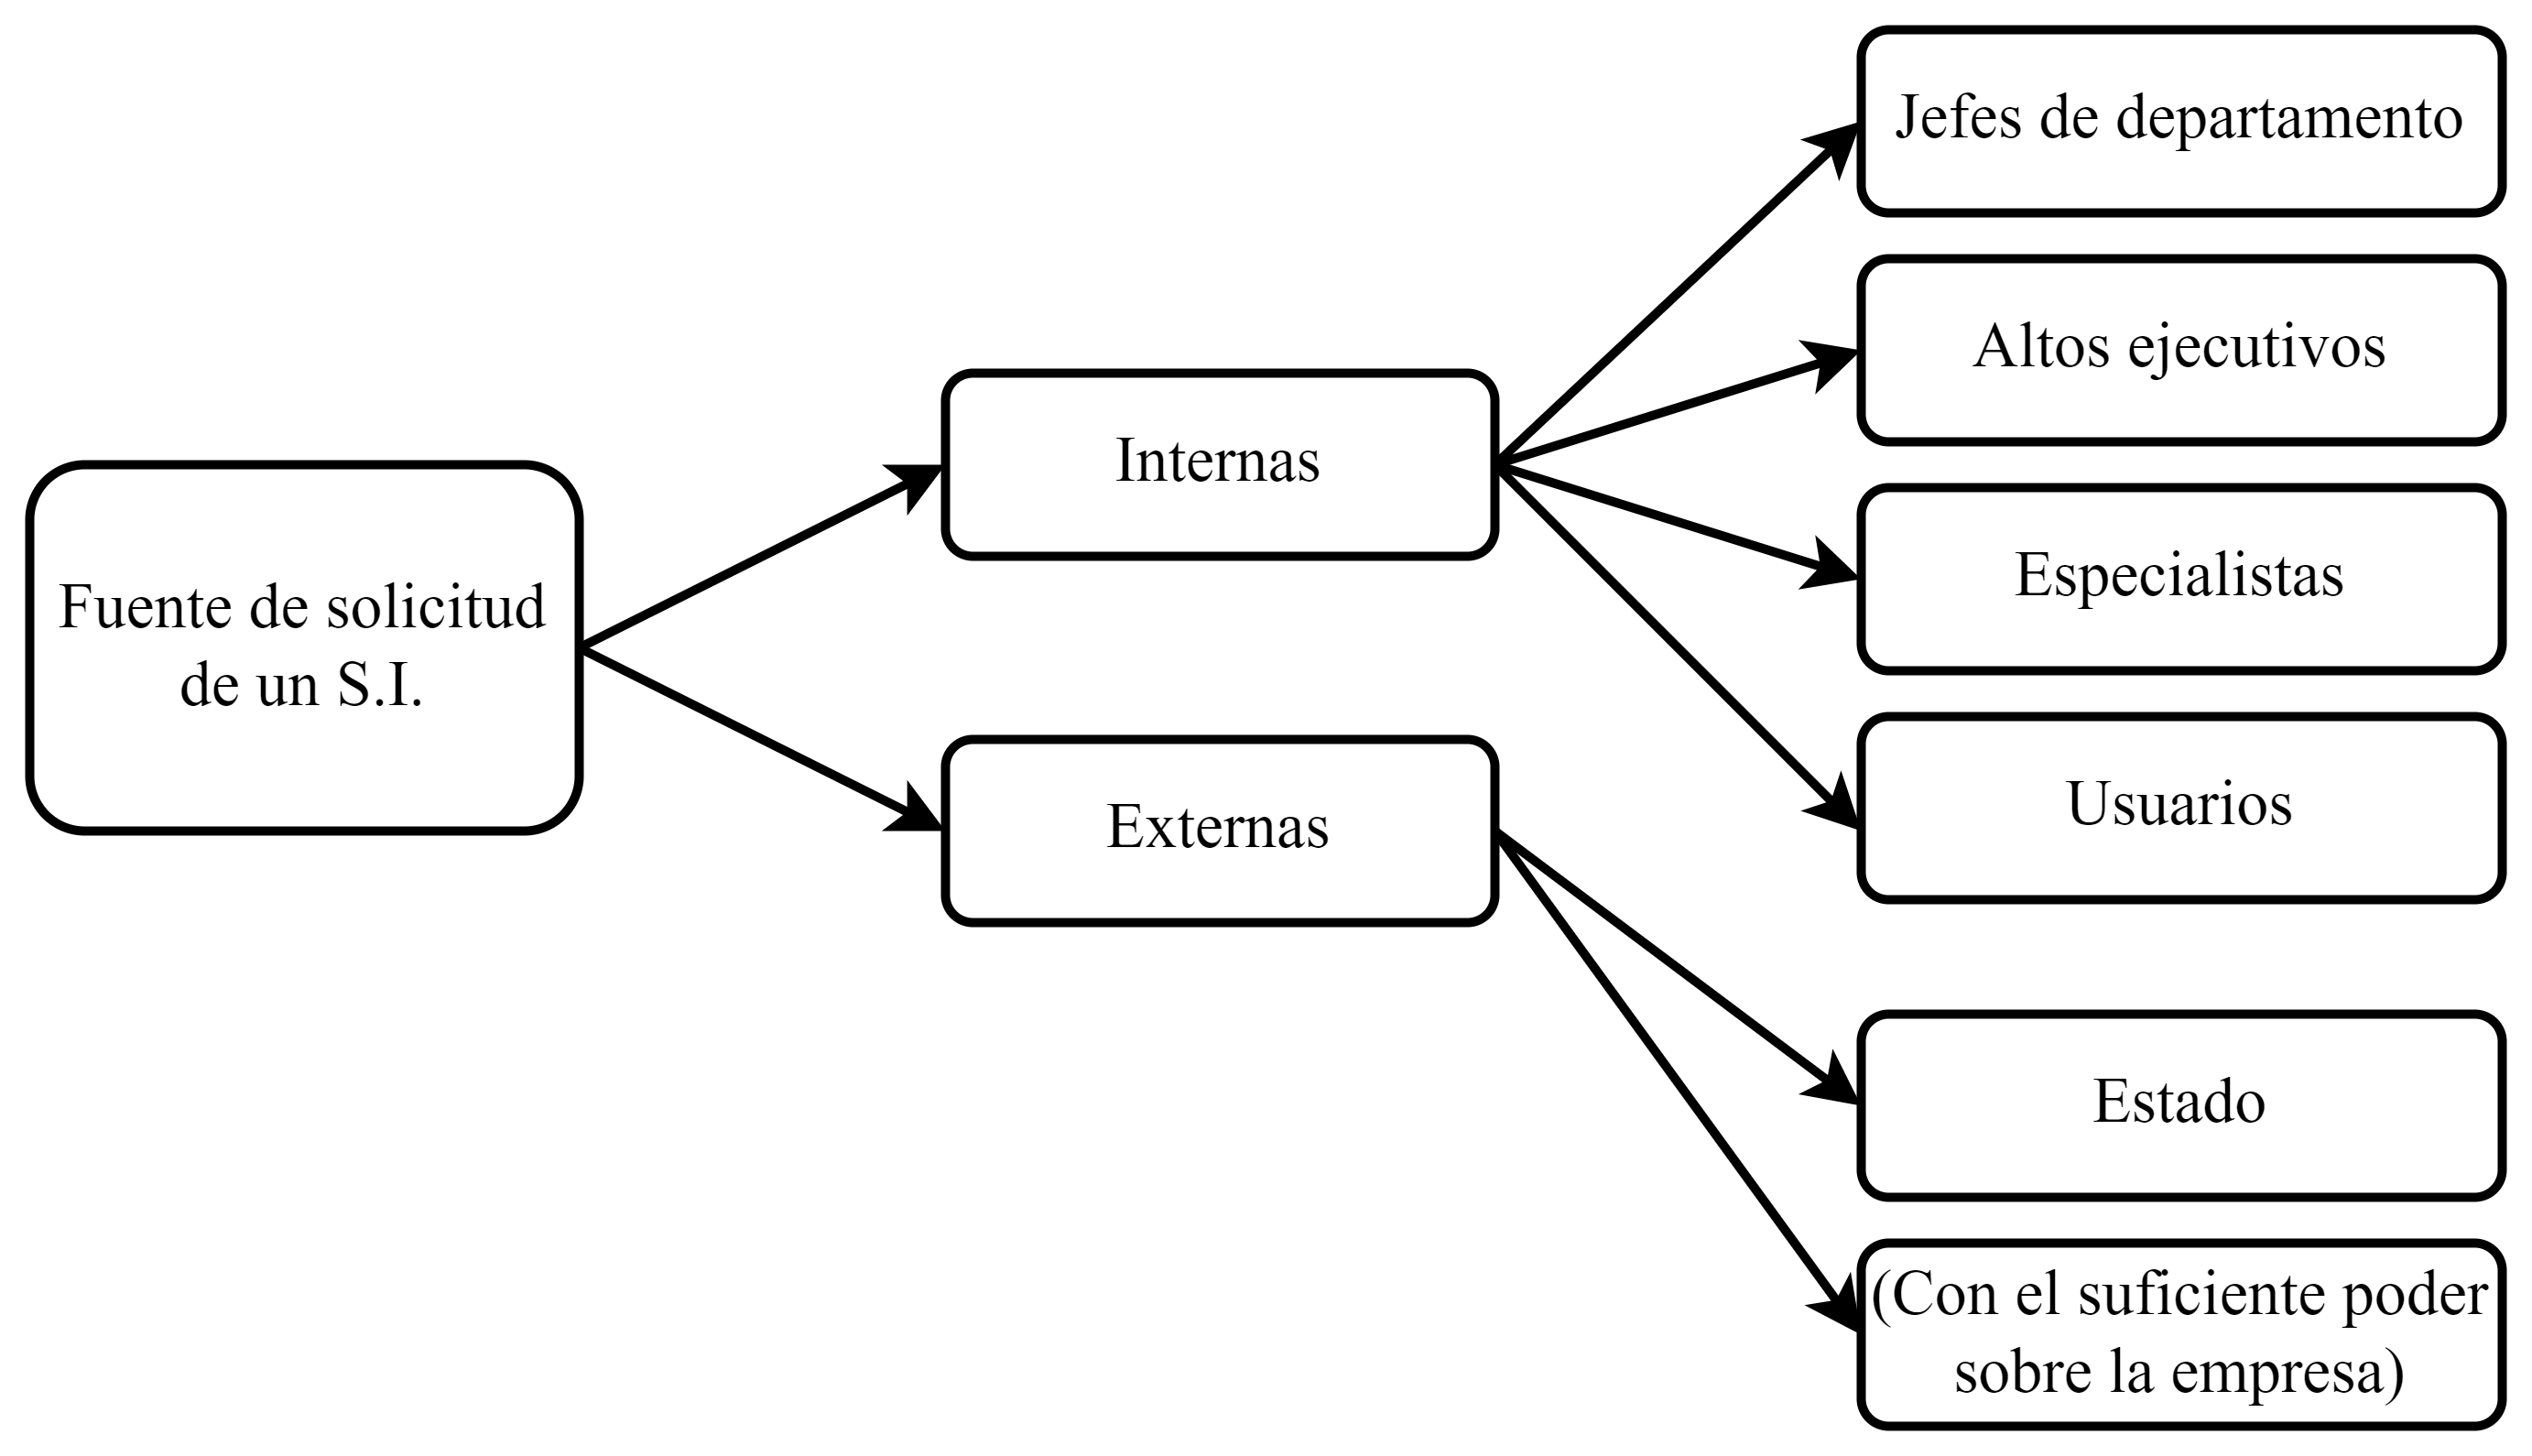
\includegraphics[width=0.85\textwidth]{diagram/FuentesSI.png}
\end{center}

\subsubsection*{Origenes de proyectos S.I.}
Razones de la creaci\'on de un proyecto S.I.:
\begin{enumerate}
    \item \textbf{Integraci\'on:} Si yo tengo sistemas aislados dentro de la misma empresa y quiero integrarlos en uno.
    \item \textbf{Velocidad de procesamiento:} Como aumentar la velocidad de procesos.
    \item \textbf{Exactitud y consistencia:} Para sistemas que manejan n\'umeros se pide exactitud.
    \item \textbf{Confiabilidad:} Un sistema puede estar disponible casi siempre, ademas de tener menos errores.
    \item \textbf{Seguridad/Confidencialidad:} Si se requiere que la informaci\'on sea accesible y confidencial para algunas personas.
    \item \textbf{Imagen:} Es algo m\'as subjetivo, para imitar a la competencia.
\end{enumerate}

\newpage
\subsubsection{Dise\~no:}
\subsubsection*{Estrategias de desarrollo:}
\subsubsection*{Ciclo de vida tradicional / Ciclo de vida lineal / M\'etodo de cascada}
Conjunto de actividades para desarrollar y poner en marcha un S.I.

Se dice:
\begin{itemize}
    \item Tradicional porque todos los informativos lo deben saber.
    \item Lineal porque las actividades se hacen linealmente sin volver atras.
    \item Cascada porque toda actividad previa le sirve a las siguientes.
\end{itemize}
\textbf{Ventajas:}
\begin{itemize}
    \item Estructura clara.
    \item Determinaci\'on r\'apida del objetivo final.
    \item Transmisi\'on efectiva de informaci\'on.
\end{itemize}
\textbf{Desventajas:}
\begin{itemize}
    \item Lento para correcci\'on de posibles errores.
    \item Excluye al cliente o al usuario final.
    \item Retrasa las pruebas dificultando los posibles cambios del cliente.
\end{itemize}

\subsubsection*{Actividades}
\begin{center}
    \begin{overpic}[width=0.8\textwidth]{diagram/Cascada.png}
        \put(1,85){\hyperlink{DF}{\phantomsection\hspace{5.8em}\raisebox{0pt}[0.4cm][0.6cm]{}}}
        \put(11,75.2){\hyperlink{EF}{\phantomsection\hspace{5.8em}\raisebox{0pt}[0.4cm][0.6cm]{}}}
        \put(20.7,65.4){\hyperlink{AS}{\phantomsection\hspace{5.8em}\raisebox{0pt}[0.4cm][0.6cm]{}}}
        \put(30.5,55.6){\hyperlink{DL}{\phantomsection\hspace{5.8em}\raisebox{0pt}[0.4cm][0.6cm]{}}}
        \put(40.3,45.8){\hyperlink{DFi}{\phantomsection\hspace{5.8em}\raisebox{0pt}[0.4cm][0.6cm]{}}}
        \put(50.1,36){\hyperlink{C}{\phantomsection\hspace{5.8em}\raisebox{0pt}[0.4cm][0.6cm]{}}}
        \put(59.9,26.2){\hyperlink{I}{\phantomsection\hspace{5.8em}\raisebox{0pt}[0.4cm][0.6cm]{}}}
        \put(69.7,16.4){\hyperlink{RPI}{\phantomsection\hspace{5.8em}\raisebox{0pt}[0.4cm][0.6cm]{}}}
        \put(79.5,6.6){\hyperlink{M}{\phantomsection\hspace{5.8em}\raisebox{0pt}[0.4cm][0.6cm]{}}}
    \end{overpic}
\end{center}

\begin{enumerate}
    \item \hypertarget{DF}{\textbf{Definición del problema:}} Se define el problema a resolver.
    \begin{itemize}
        \item Estudio de la situación actual.
        
        \item Identificación del problema.
        
        \item Objetivos del sistema: Se debe apuntar a resolver el problema de la situaci\'on actual.
        
        Los objetivos deben comenzar por un verbo (Construir, Proponer, ...).
        \begin{itemize}
            \item Objetivo general: Se refiere a la soluci\'on del problema.
            
            \item Objetivos espec\'ificos: Se refieren a las partes del problema.
        \end{itemize}
        
        \item Limites del sistema: Se definen limites para evitar que el proyecto se salga de control.
        
        \item Ámbito del sistema: ¿El sistema apoya al t\'ecnico, empresarial u operativo? (A que zona de la pirámide de Anthony).
        
        \item Bases del sistema (Aspectos legales).
        
        \item Requerimientos del sistema (Que se espera del sistema).
        \begin{itemize}
            \item Requerimientos de información (Que información maneja el sistema).
            
            \item Requerimientos técnicos (Hardware, software y recursos humanos).
            
            \item Requerimientos funcionales (Estadísticas, gráficas y cosas que el sistema puede crear con los datos que maneja).
            
            \item Requerimientos de seguridad (Claves y niveles de acceso).
        \end{itemize}
    \end{itemize}

    \item \hypertarget{EF}{\textbf{Estudio de factibilidad:}} Se estudia si es factible realizar el proyecto. Si uno de los siguientes 3 estudios no se cumple ya no es factible:
    \begin{itemize}
        \item Estudio de factibilidad operativo.
        \begin{itemize}
            \item ¿La gente est\'a de acuerdo o interesada en el S.I.?
            \item ¿La operaci\'on o S.I. afecta en otras \'areas?
        \end{itemize}

        \item Estudio de factibilidad técnico.
        \begin{itemize}
            \item ¿Se tiene la tecnolog\'ia(Hardware, Software) necesaria?
            \item ¿Se tiene el personal(RRHH) necesario?
            \item Hay veces que se puede seguir con el proyecto, dejando solo lo primordial e ir integrando lo faltante a futuro.
        \end{itemize}
        \item Estudio de factibilidad económico: Establecimiento de costos y beneficios. $(Costos < Beneficios)$.
    \end{itemize}
    \item \hypertarget{AS}{\textbf{Análisis del sistema:}} Una vez se confirma la factibilidad del proyecto se proceden a analizar las entradas, procesos y salidas que conformaran el sistema para su funcionamiento.
    \item \hypertarget{DL}{\textbf{Diseño lógico:}} Se diseña el sistema en base a los requerimientos del sistema. Este diseño puede ser de 4 tipos:
        \begin{enumerate}
            \item Diagrama de flujo de datos (DFD): Sirven para modelar procesos y muestra como se mueve la información.
            \item Diseño de procedimientos administrativos: Elementos necesarios para llevar a cabo una función administrativa resumido en un documento.
            
            \newpage
            \item Diseño de sistemas de codificación: Representación en caracteres de la información para evitar el uso de largas cadenas de codificación.\newline
            Existen varios tipos de codificación:
            \begin{itemize}
                \item Secuencial: Cada elemento tiene un número y se ordenan de menor a mayor. Fácil de codificar pero dificulta la búsqueda de datos.
                \item Por bloque: Se agrupan los elementos en bloques y se les asigna un número. Facilita la búsqueda de datos como en un indice.
                \item De consonantes: Se basa en la eliminación de las consonantes después de la primera consonante de cada palabra.
                \begin{tcolorbox}[colback=green!10!white,colframe=green!75!black,title=Ejemplo de codificación de consonantes]
                    \begin{center}
                        \begin{tabular}{|c|c|}
                            \hline
                            \textbf{Nombre} & \textbf{Codificación} \\ \hline
                            Ingeniería & Ingnr \\ \hline
                            Informática & Infrm \\ \hline
                            Computación & Cmptc \\ \hline
                        \end{tabular}
                    \end{center}
                \end{tcolorbox}
                \item Nemotécnico: Uno de los tipos de codificación mas usados, se basa en la creación de una palabra clave para cada elemento.
                Sin embargo dependiendo de la codificación esta palabra clave puede significar mas de una cosa, lo que nunca puede pasar.
                \begin{tcolorbox}[colback=green!10!white,colframe=green!75!black,title=Ejemplo de codificación Nemotécnica]
                    \begin{center}
                        \begin{tabular}{|c|c|}
                            \hline
                            \textbf{Nombre} & \textbf{Codificación} \\ \hline
                            Universidad del Bio Bio & UBB \\ \hline
                            Universidad de Concepción & UDEC \\ \hline
                            Universidad de Santiago & USACH \\ \hline
                        \end{tabular}
                    \end{center}
                \end{tcolorbox}
                \item Por grupos: Se agrupan elementos en grupos que poe si solos tienen un significado, pero el conjunto de estos grupos también tiene un significado. Facilita la búsqueda de datos al igual que un indice.
                \begin{tcolorbox}[colback=green!10!white,colframe=green!75!black,title=Ejemplo de codificación Por grupos]
                    \begin{center}
                        \begin{tabular}{|c|c|}
                            \hline
                            \textbf{Nombre} & \textbf{Codificación} \\ \hline
                            Ingeniería & T \\ \hline
                            Civil & 1 \\ \hline
                            En Ejecución & 2 \\ \hline
                            Informática & I0 \\ \hline
                            Biomédica & B0 \\ \hline
                        \end{tabular}
                        \\[0.5cm]
                        T1I0 $\rightarrow$ Ingeniería Civil Informática \\
                        T1B0 $\rightarrow$ Ingeniería Civil Biomédica \\
                        T2I0 $\rightarrow$ Ingeniería En Ejecución Informática
                    \end{center}
                \end{tcolorbox}
            \end{itemize}

            \newpage
            \item Diseño conceptual E/S (Entrada/Salida): Se diseña la forma en que se ingresaran los datos al sistema y como se mostraran los resultados.
            \begin{figure}[H]
                \centering
                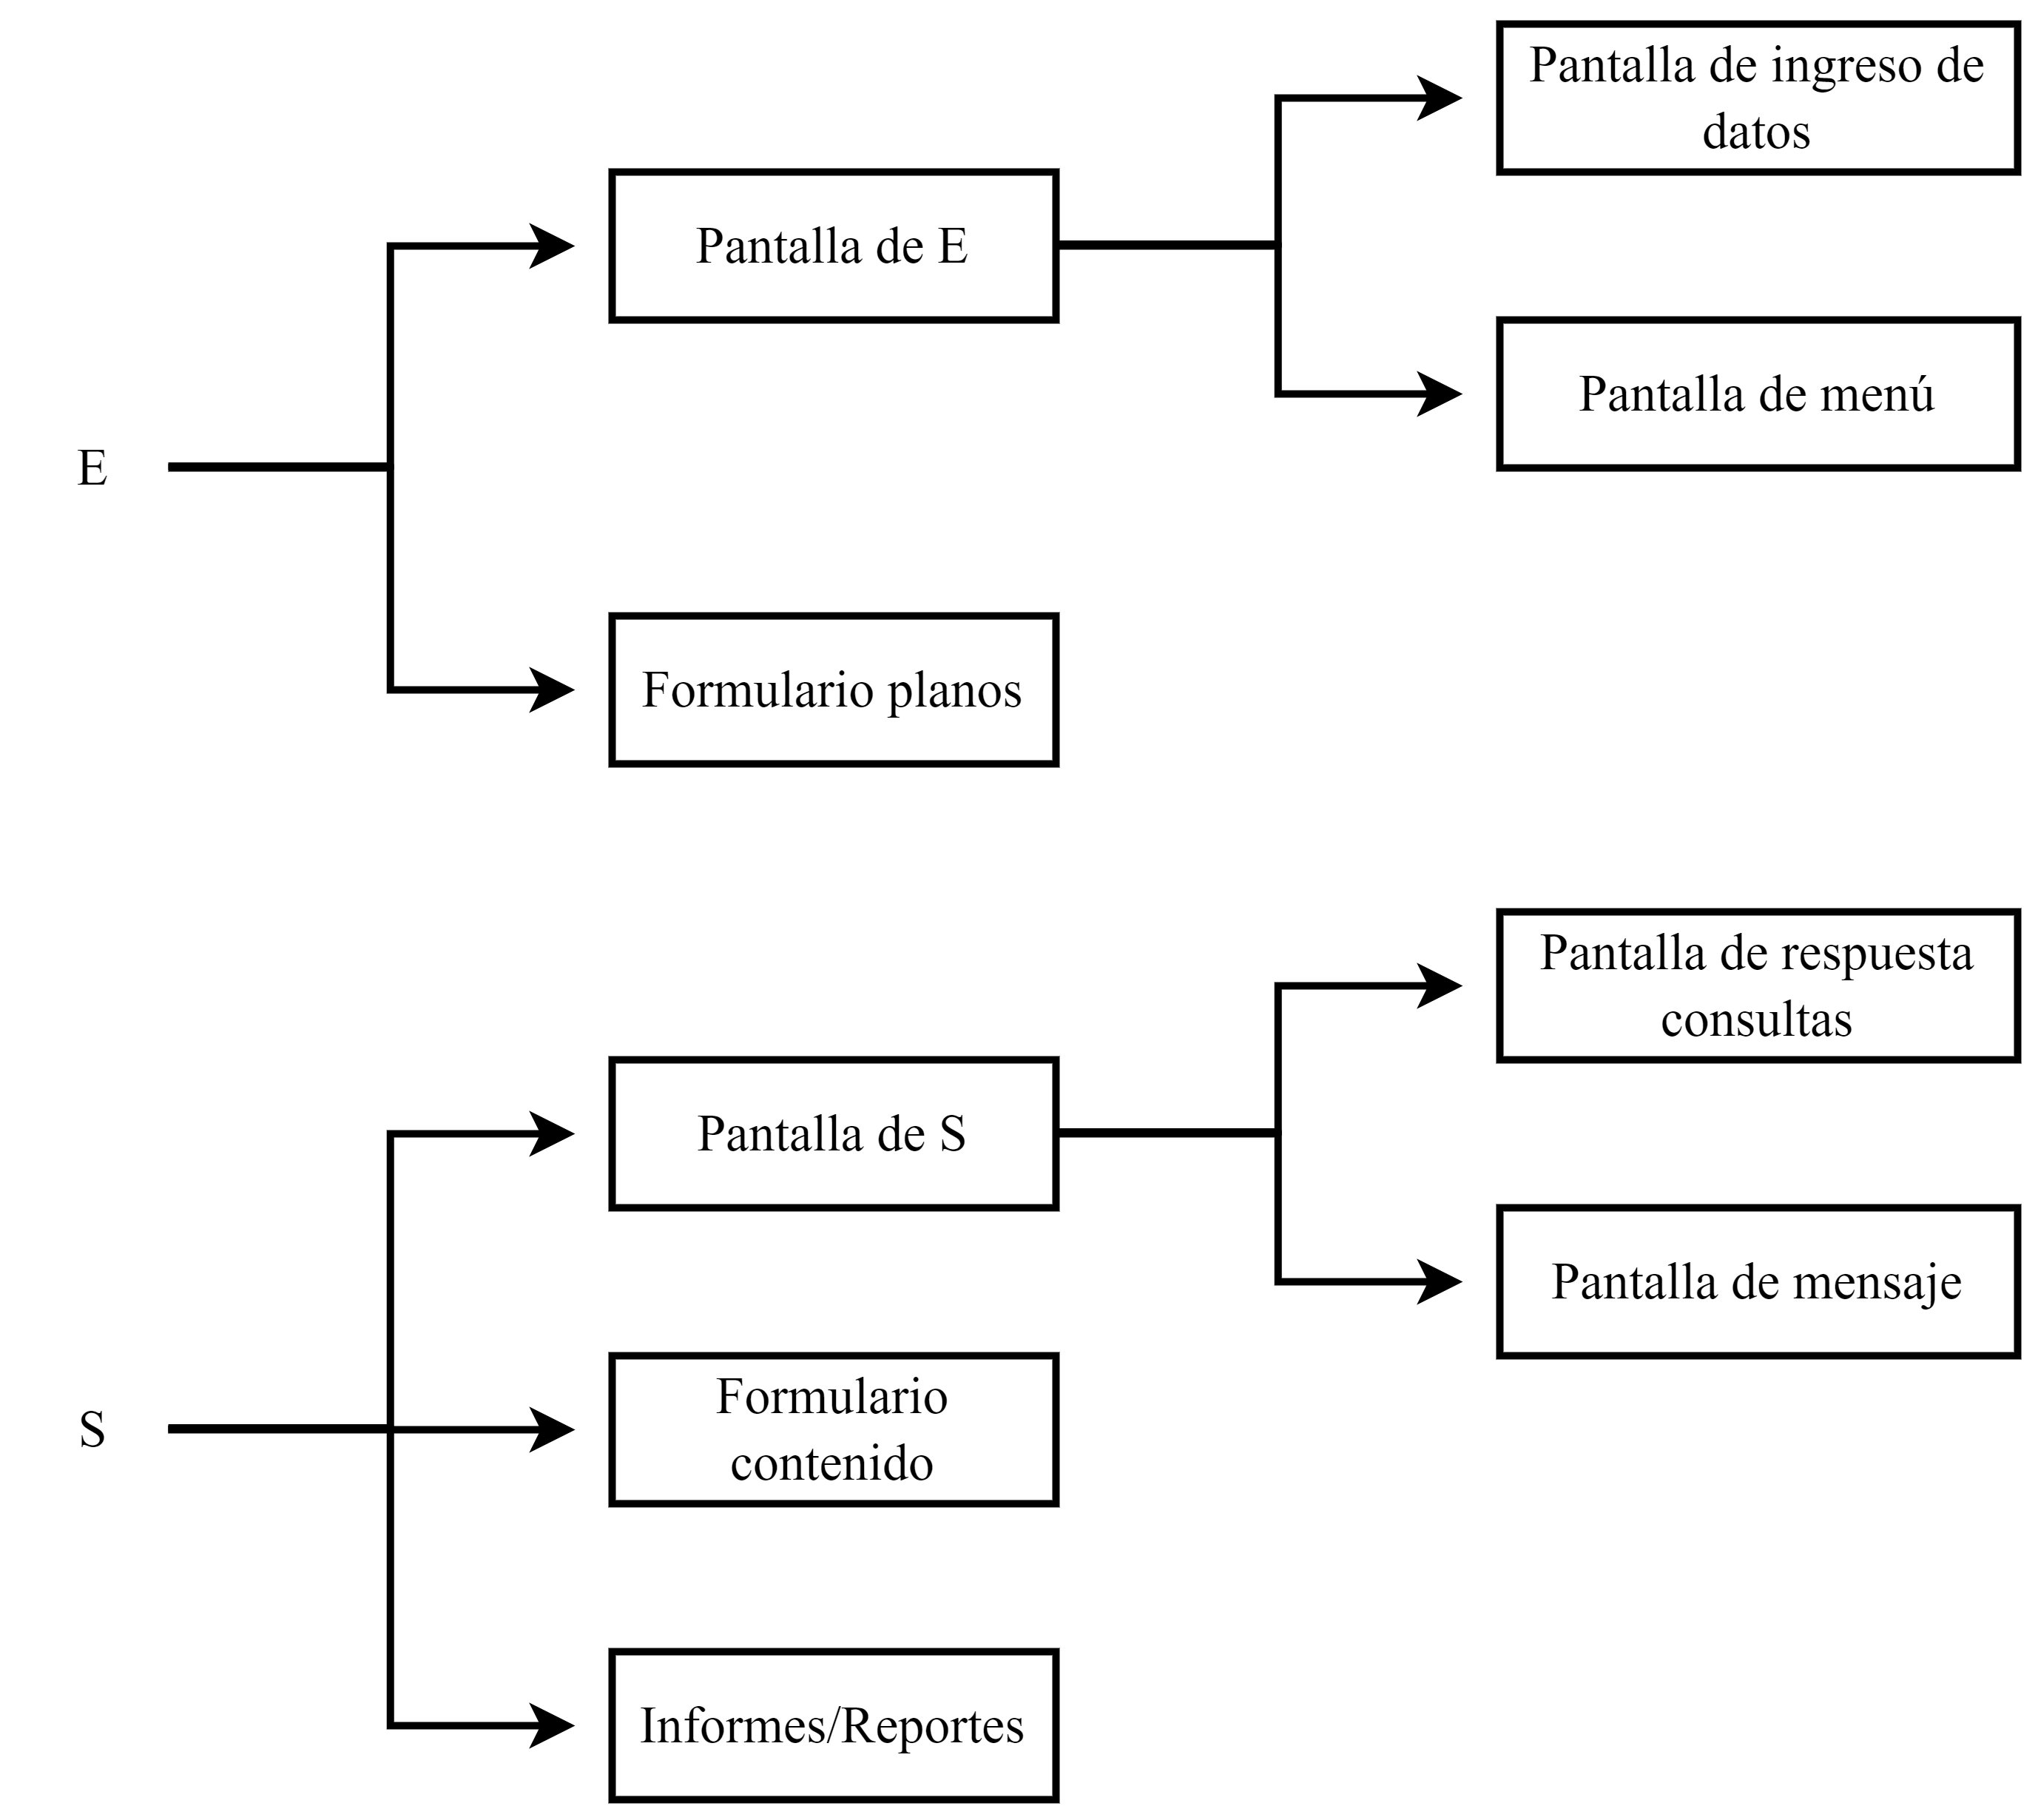
\includegraphics[width=0.8\textwidth]{diagram/EntradaSalida.png}
            \end{figure}
        \end{enumerate}
        
        \item \hypertarget{DFi}{\textbf{Diseño físico:}} Se diseña el sistema en base a la información que se tiene como objetivo manejar.
        \begin{itemize}
            \item Diseño físico E/S.
            \item Diseño de base de datos (MER/Modelo de datos).
            \item Diseño jerarquía de menus.
        \end{itemize}
    \item \label{item:ConsCas} \hypertarget{C}{\textbf{Construcción:}} Punto en el cual se procede en la selección del lenguaje sobre el cual trabajaremos, el que utilizaremos para crear un programa y someterlo a pruebas de funcionamiento.
    
    El objetivo de probar el programa es lograr un programa fiable y que cumpla con los requerimientos del sistema (que no se caiga) y asi poder entregar un sistema completamente funcional.
    
    \newpage
    \item \label{item:ImplCas} \hypertarget{I}{\textbf{Implementación:}} 
    \begin{itemize}
        \item Poblado de base de datos: Ingreso de datos necesarios para el funcionamiento del sistema, siendo estos datos requerimientos de información.
        \item Entrenamiento/capacitación de usuarios: Enseñar al usuario a usar los datos del sistema.
        \begin{itemize}
            \item Usuarios a capacitar.
            \item Responsable capacitación.
            \item Recursos necesarios.
            \item Plan de capacitación. 
        \end{itemize}
        \item Puesta en marcha: Poner en funcionamiento el sistema, existen 4 formas de poner en marcha un sistema:            
        \begin{itemize}
            \item Inmediata: Apenas finaliza el sistema anterior, el nuevo sistema entra en funcionamiento (Opción mas arriesgada al momento de poner a prueba el nuevo sistema).
            \begin{figure}[H]
                \centering
                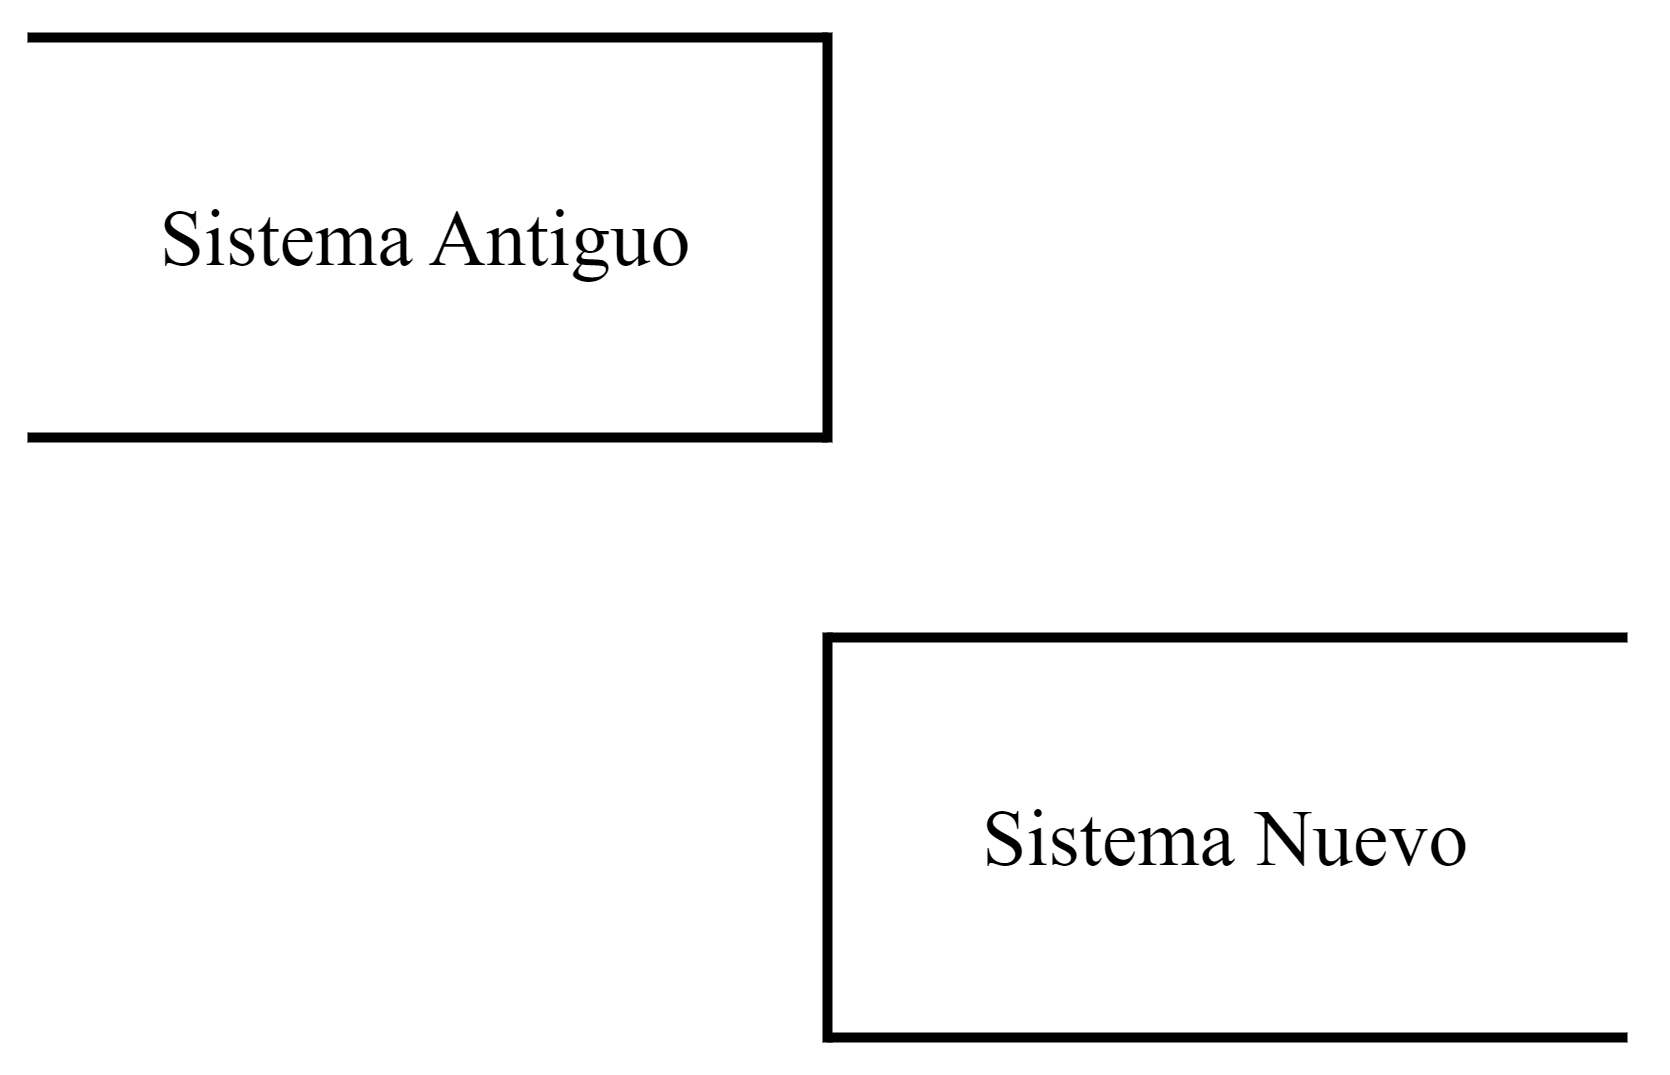
\includegraphics[width=0.6\textwidth]{diagram/MarchaInmediata.png}
            \end{figure}
            \item Paralela: Mientras el sistema antiguo sigue en funcionamiento, el nuevo sistema se va implementando por completo (Opción mas segura pero consume muchos recursos).
            \begin{figure}[H]
                \centering
                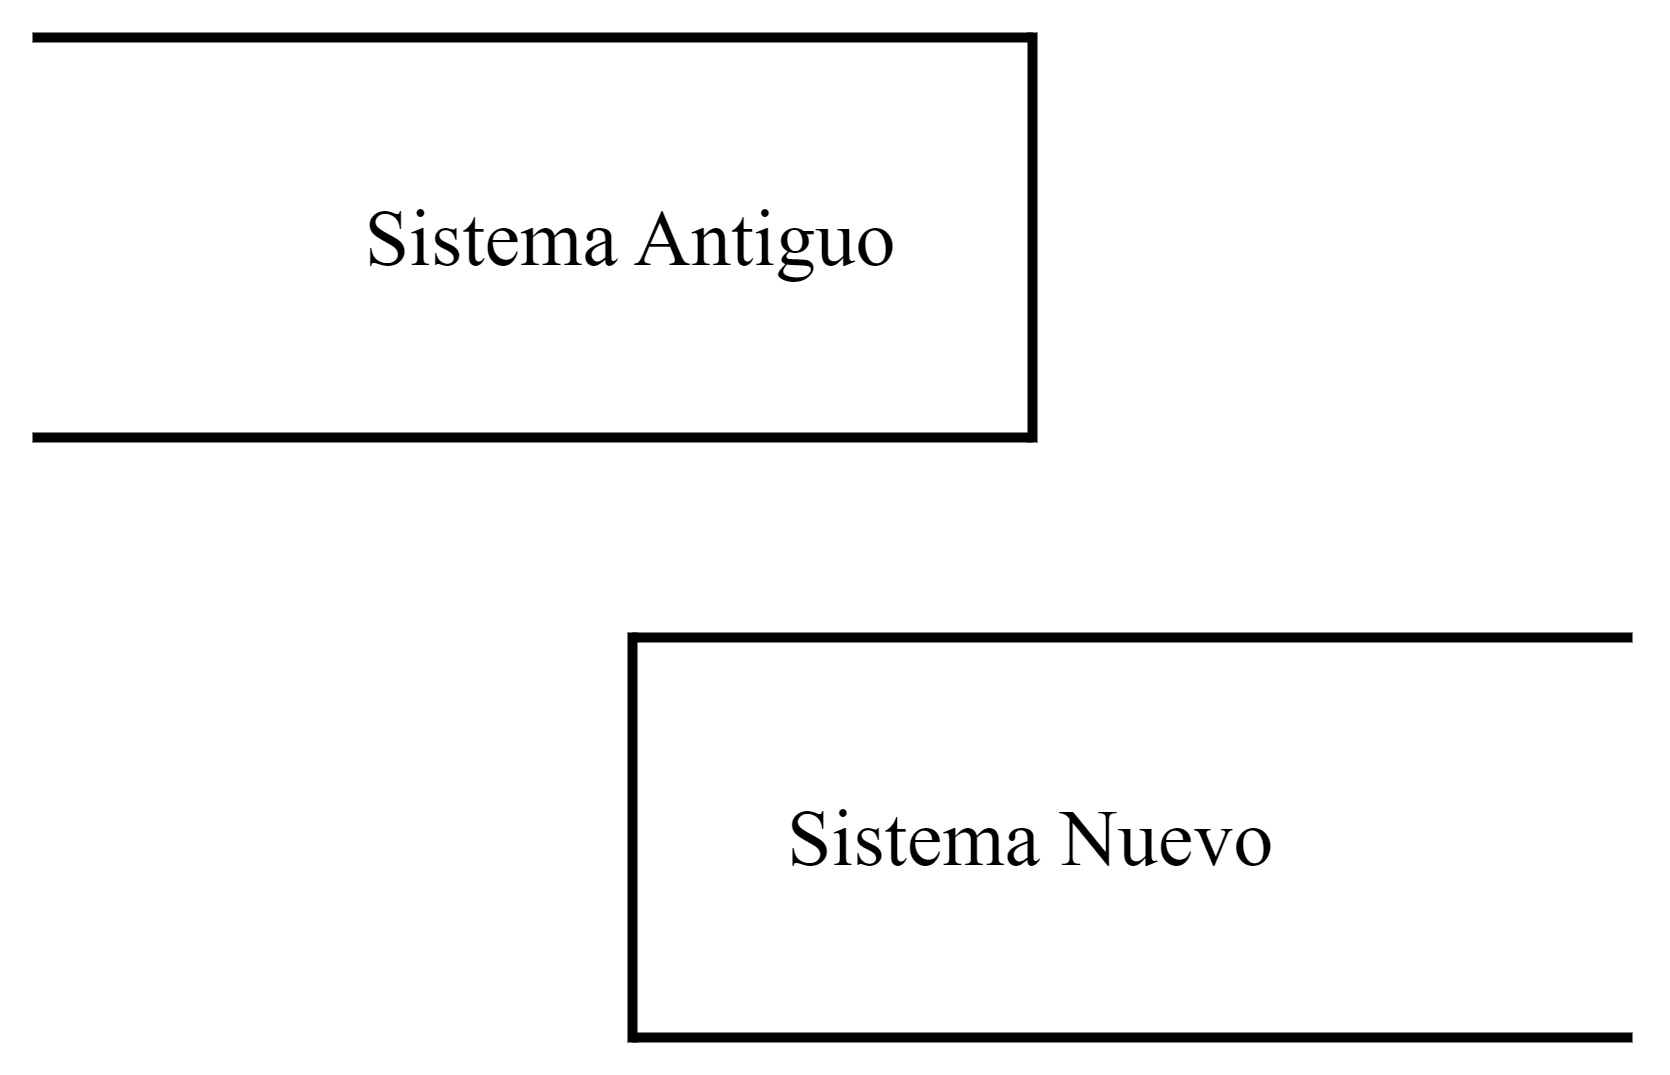
\includegraphics[width=0.6\textwidth]{diagram/MarchaParalela.png}
            \end{figure}
            \item Piloto: Se implementa el sistema en una parte de la empresa para ver como funciona (Opción intermedia).
            \begin{figure}[H]
                \centering
                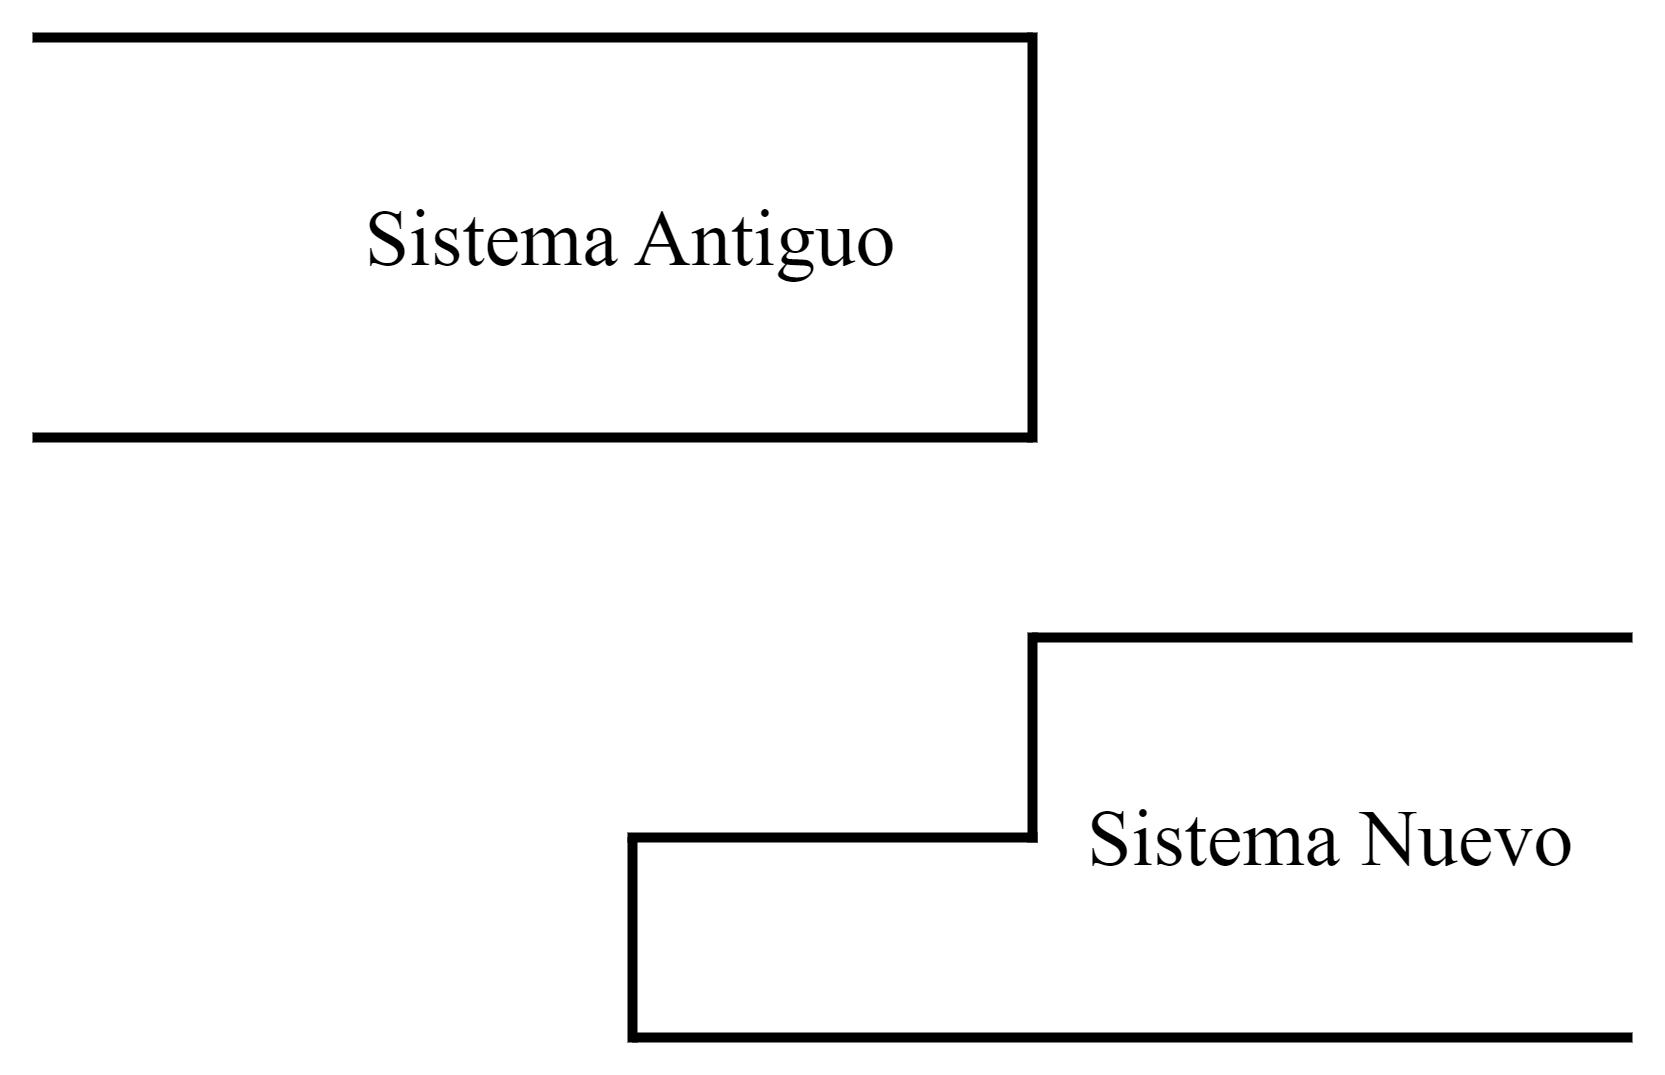
\includegraphics[width=0.6\textwidth]{diagram/MarchaPiloto.png}
            \end{figure}
            \item Gradual: Se implementa el sistema por partes mientras el antiguo sigue en funcionamiento (Opción segura pero no al nivel de la paralela).
            \begin{figure}[H]
                \centering
                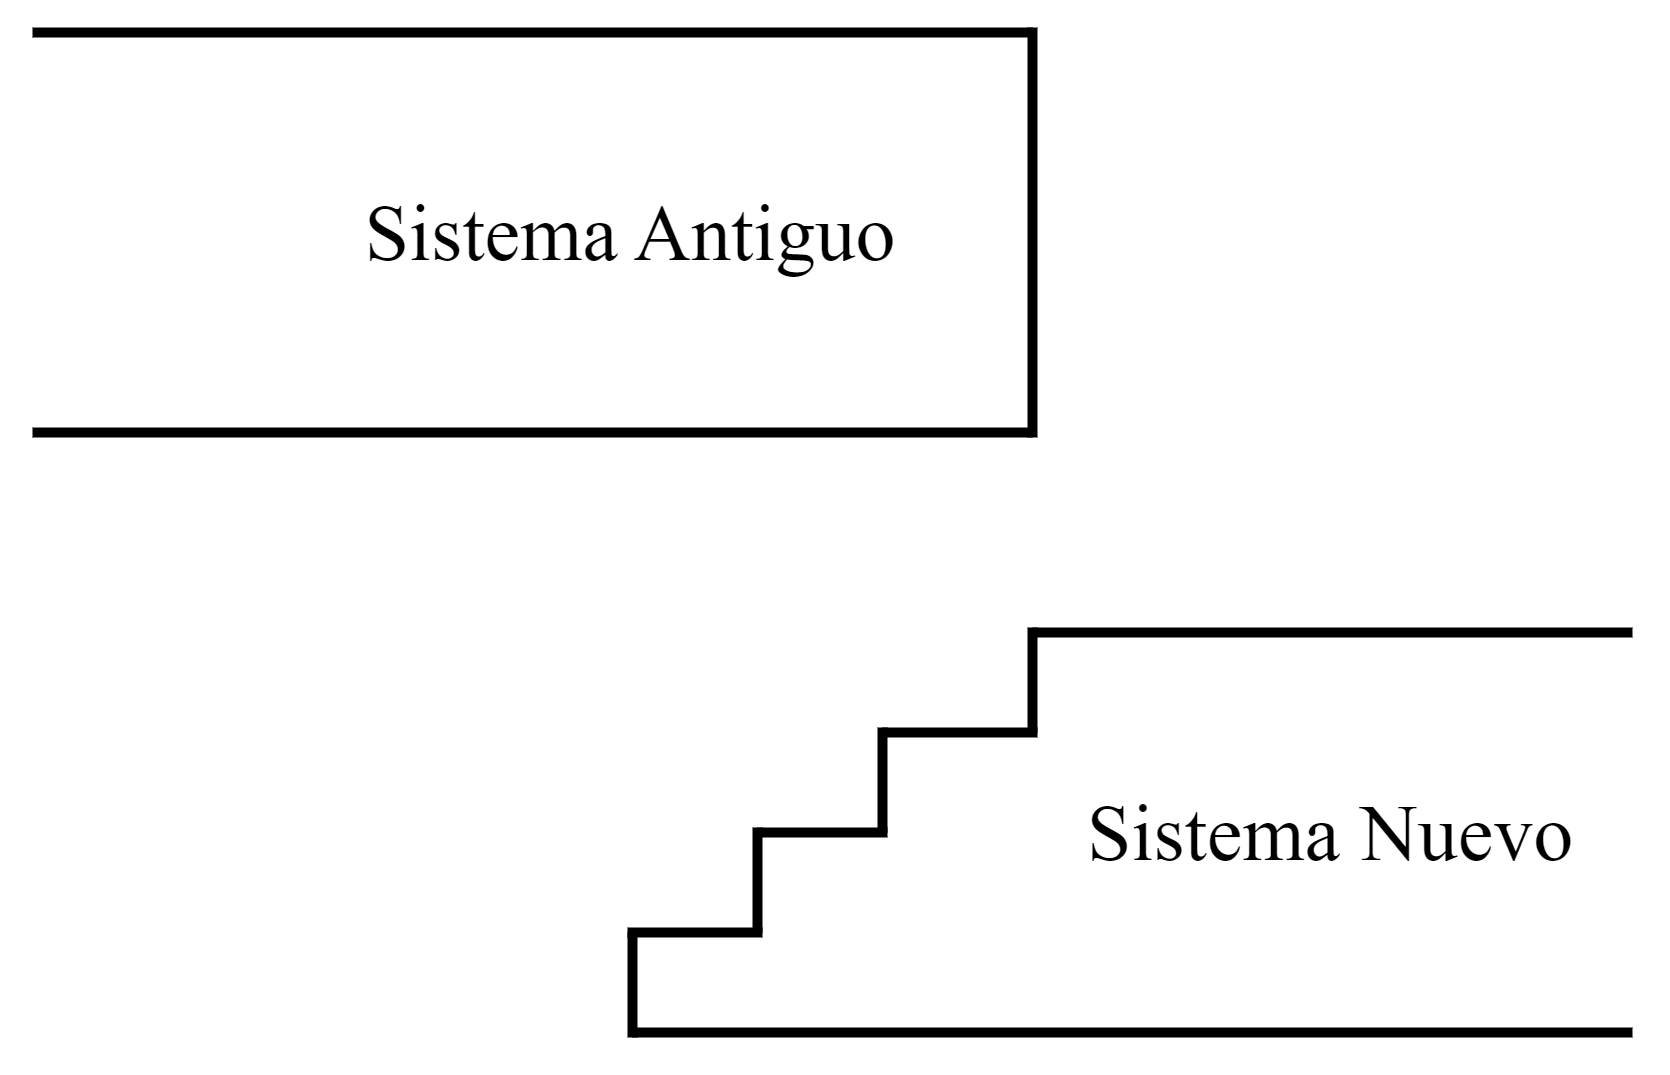
\includegraphics[width=0.6\textwidth]{diagram/MarchaGradual.png}
            \end{figure}
        \end{itemize}
    \end{itemize}

    \item \hypertarget{RPI}{\textbf{Revisión post-implementación:}} Revision del funcionamiento correcto del sistema instalado.
    
    \item \hypertarget{M}{\textbf{Mantención:}} Proceso de corrección de errores y mejoras del sistema. Existen 4 tipos de mantenimiento:
    \begin{itemize}
        \item Preventiva: Se realiza antes de que ocurra un error.
        \item Correctiva: Se realiza después de que ocurra un error.
        \item Perfectiva: Se realiza para mejorar el sistema.
        \item Adaptativa: Se realiza para adaptar el sistema a cambios en el entorno y sus nuevas tecnologías.
    \end{itemize}
\end{enumerate}

\newpage
\subsubsection*{Prototipos}
\noindent Alternativa al ciclo de vida tradicional, se basa en la creación de un prototipo para que el cliente pueda ver como se verá el sistema final.
\begin{itemize}
    \item \textbf{Ventajas:}
    \begin{itemize}
        \item Se puede ver el sistema antes de que este terminado.
        \item Se pueden hacer cambios antes de que el sistema este terminado.
        \item Se puede ver si el sistema cumple con los requerimientos.
        \item Se determina mas rápidamente la viabilidad del proyecto.
    \end{itemize}
    \item \textbf{Desventajas:}
    \begin{itemize}
        \item Puede ser costoso.
        \item Puede ser lento.
        \item Puede ser difícil de implementar.
        \item El usuario puede no saber que es lo que quiere.
        \item El usuario debe estar presente en todo momento.
    \end{itemize}
\end{itemize}
\begin{center}
    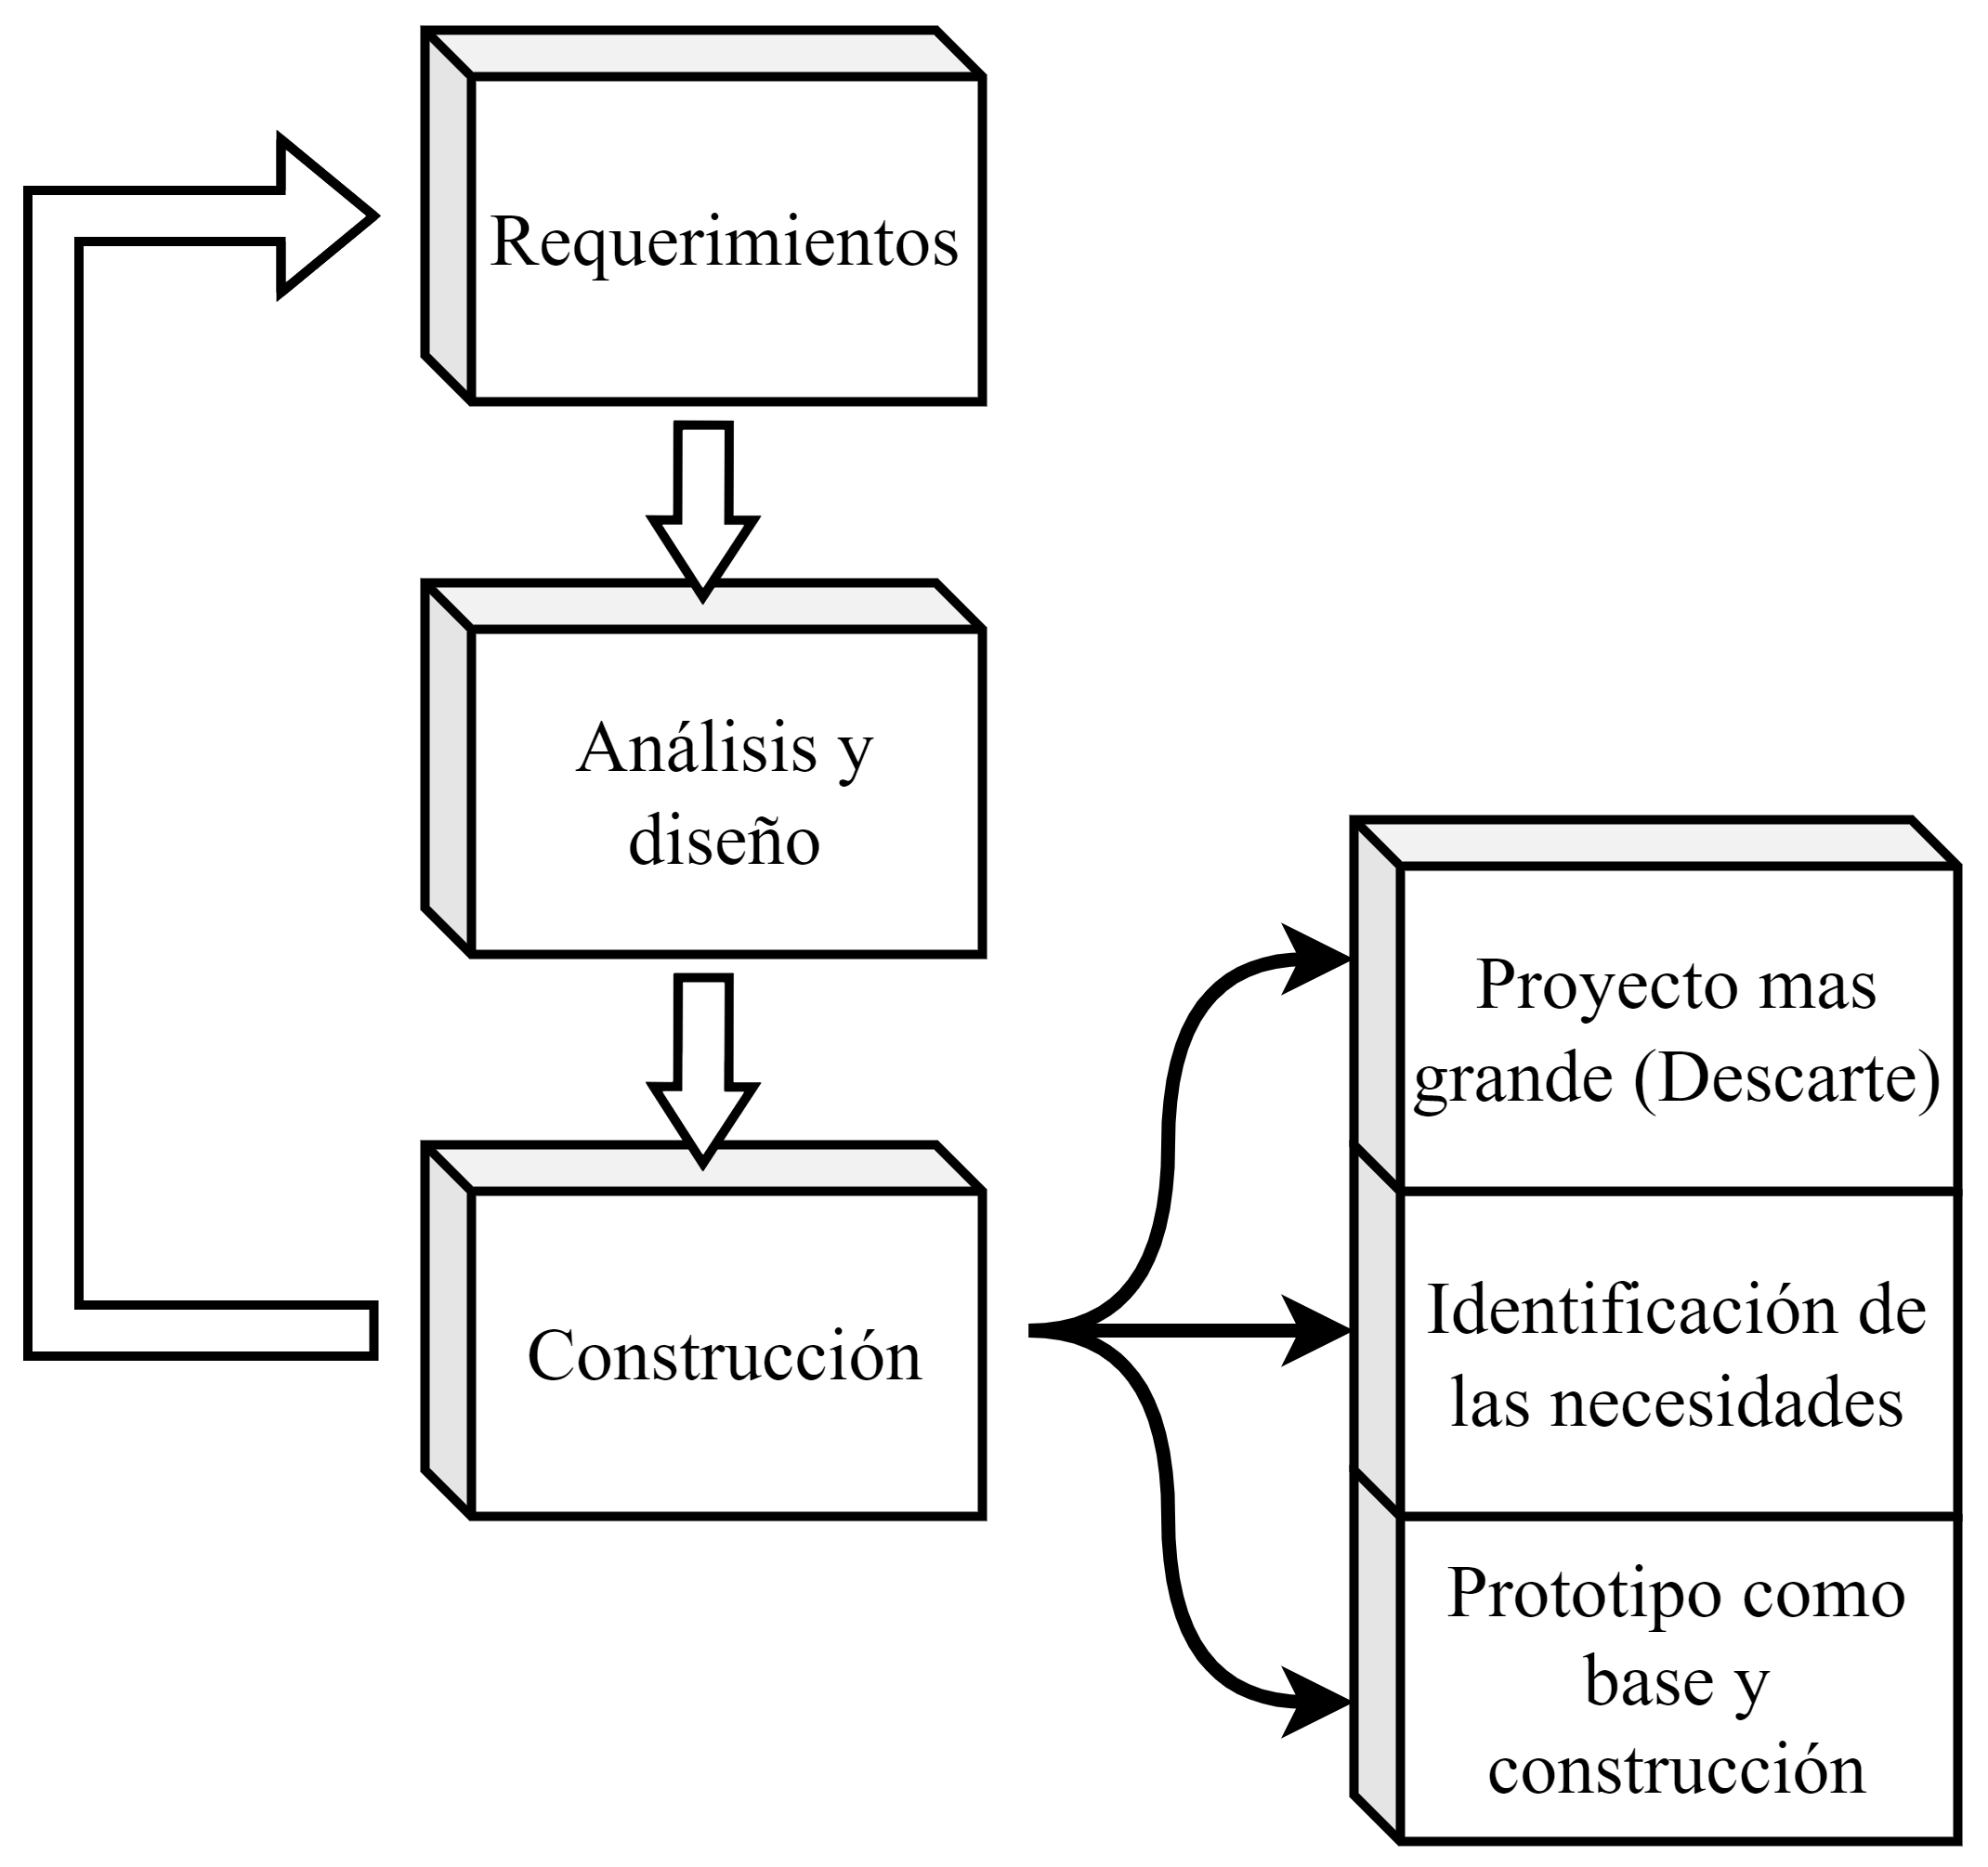
\includegraphics[width=0.8\textwidth]{diagram/Prototipos.png}
\end{center}

\newpage
\noindent En la creación de un prototipo se deben seguir los siguientes pasos:
\begin{enumerate}
    \item \textbf{Definición de requerimientos:} Se definen los requerimientos del sistema.
    
    \item \textbf{Diseño del prototipo:} Se diseña el prototipo.
    
    \item \label{item:ConsPro} \textbf{Construcción del prototipo:} Se construye el prototipo.
    
    En este punto del proceso se pueden dar 4 situaciones:
    
    \begin{enumerate}
        \item La construcción del prototipo no es la esperada por lo que se vuelve al diseño del prototipo.
        
        \item El prototipo no es el esperado pero ya se identificaron las necesidades del usuario.
        
        \item El proyecto resulta ser mas grande de lo esperado por lo tanto se descarta el proyecto.
        
        \item \label{subitem:ImplPro} El prototipo es el esperado por lo que se pasa a la etapa de construcción tomando el prototipo como base.
    \end{enumerate}
\end{enumerate}

\subsubsection{Construcci\'on}
Como se mencion\'o anteriormente en las partes especificas de cada estrategia.

Para la estrategia:
\begin{itemize}
    \item C.V.T: En la actividad \ref{item:ConsCas} de la cascada se selecciona el lenguaje de programaci\'on, creando un programa para luego someterlo a pruebas para que el sistema sea complentamente funcional y fiable.
    \item Prototipos: En el paso \ref{item:ConsPro} se construye el prototipo, siguiendo el procedimiento de las 4 situaciones para comprobar si se sigue iterando sobre el prototipo.
\end{itemize}

\subsubsection{Implementaci\'on}
Como se mencion\'o anteriormente en las partes especificas de cada estrategia.

Para la estrategia:
\begin{itemize}
    \item C.V.T: En la actividad \ref{item:ImplCas} de la cascada se hace el poblado de la BD, entrenamiento / capacitaci\'on de usuarios y la puesta en marcha.
    \item Prototipos: En el paso \ref{subitem:ImplPro} se construye el S.I., utilizando el prototipo como una base.
\end{itemize}

\newpage
\subsection{???}
\begin{center}
    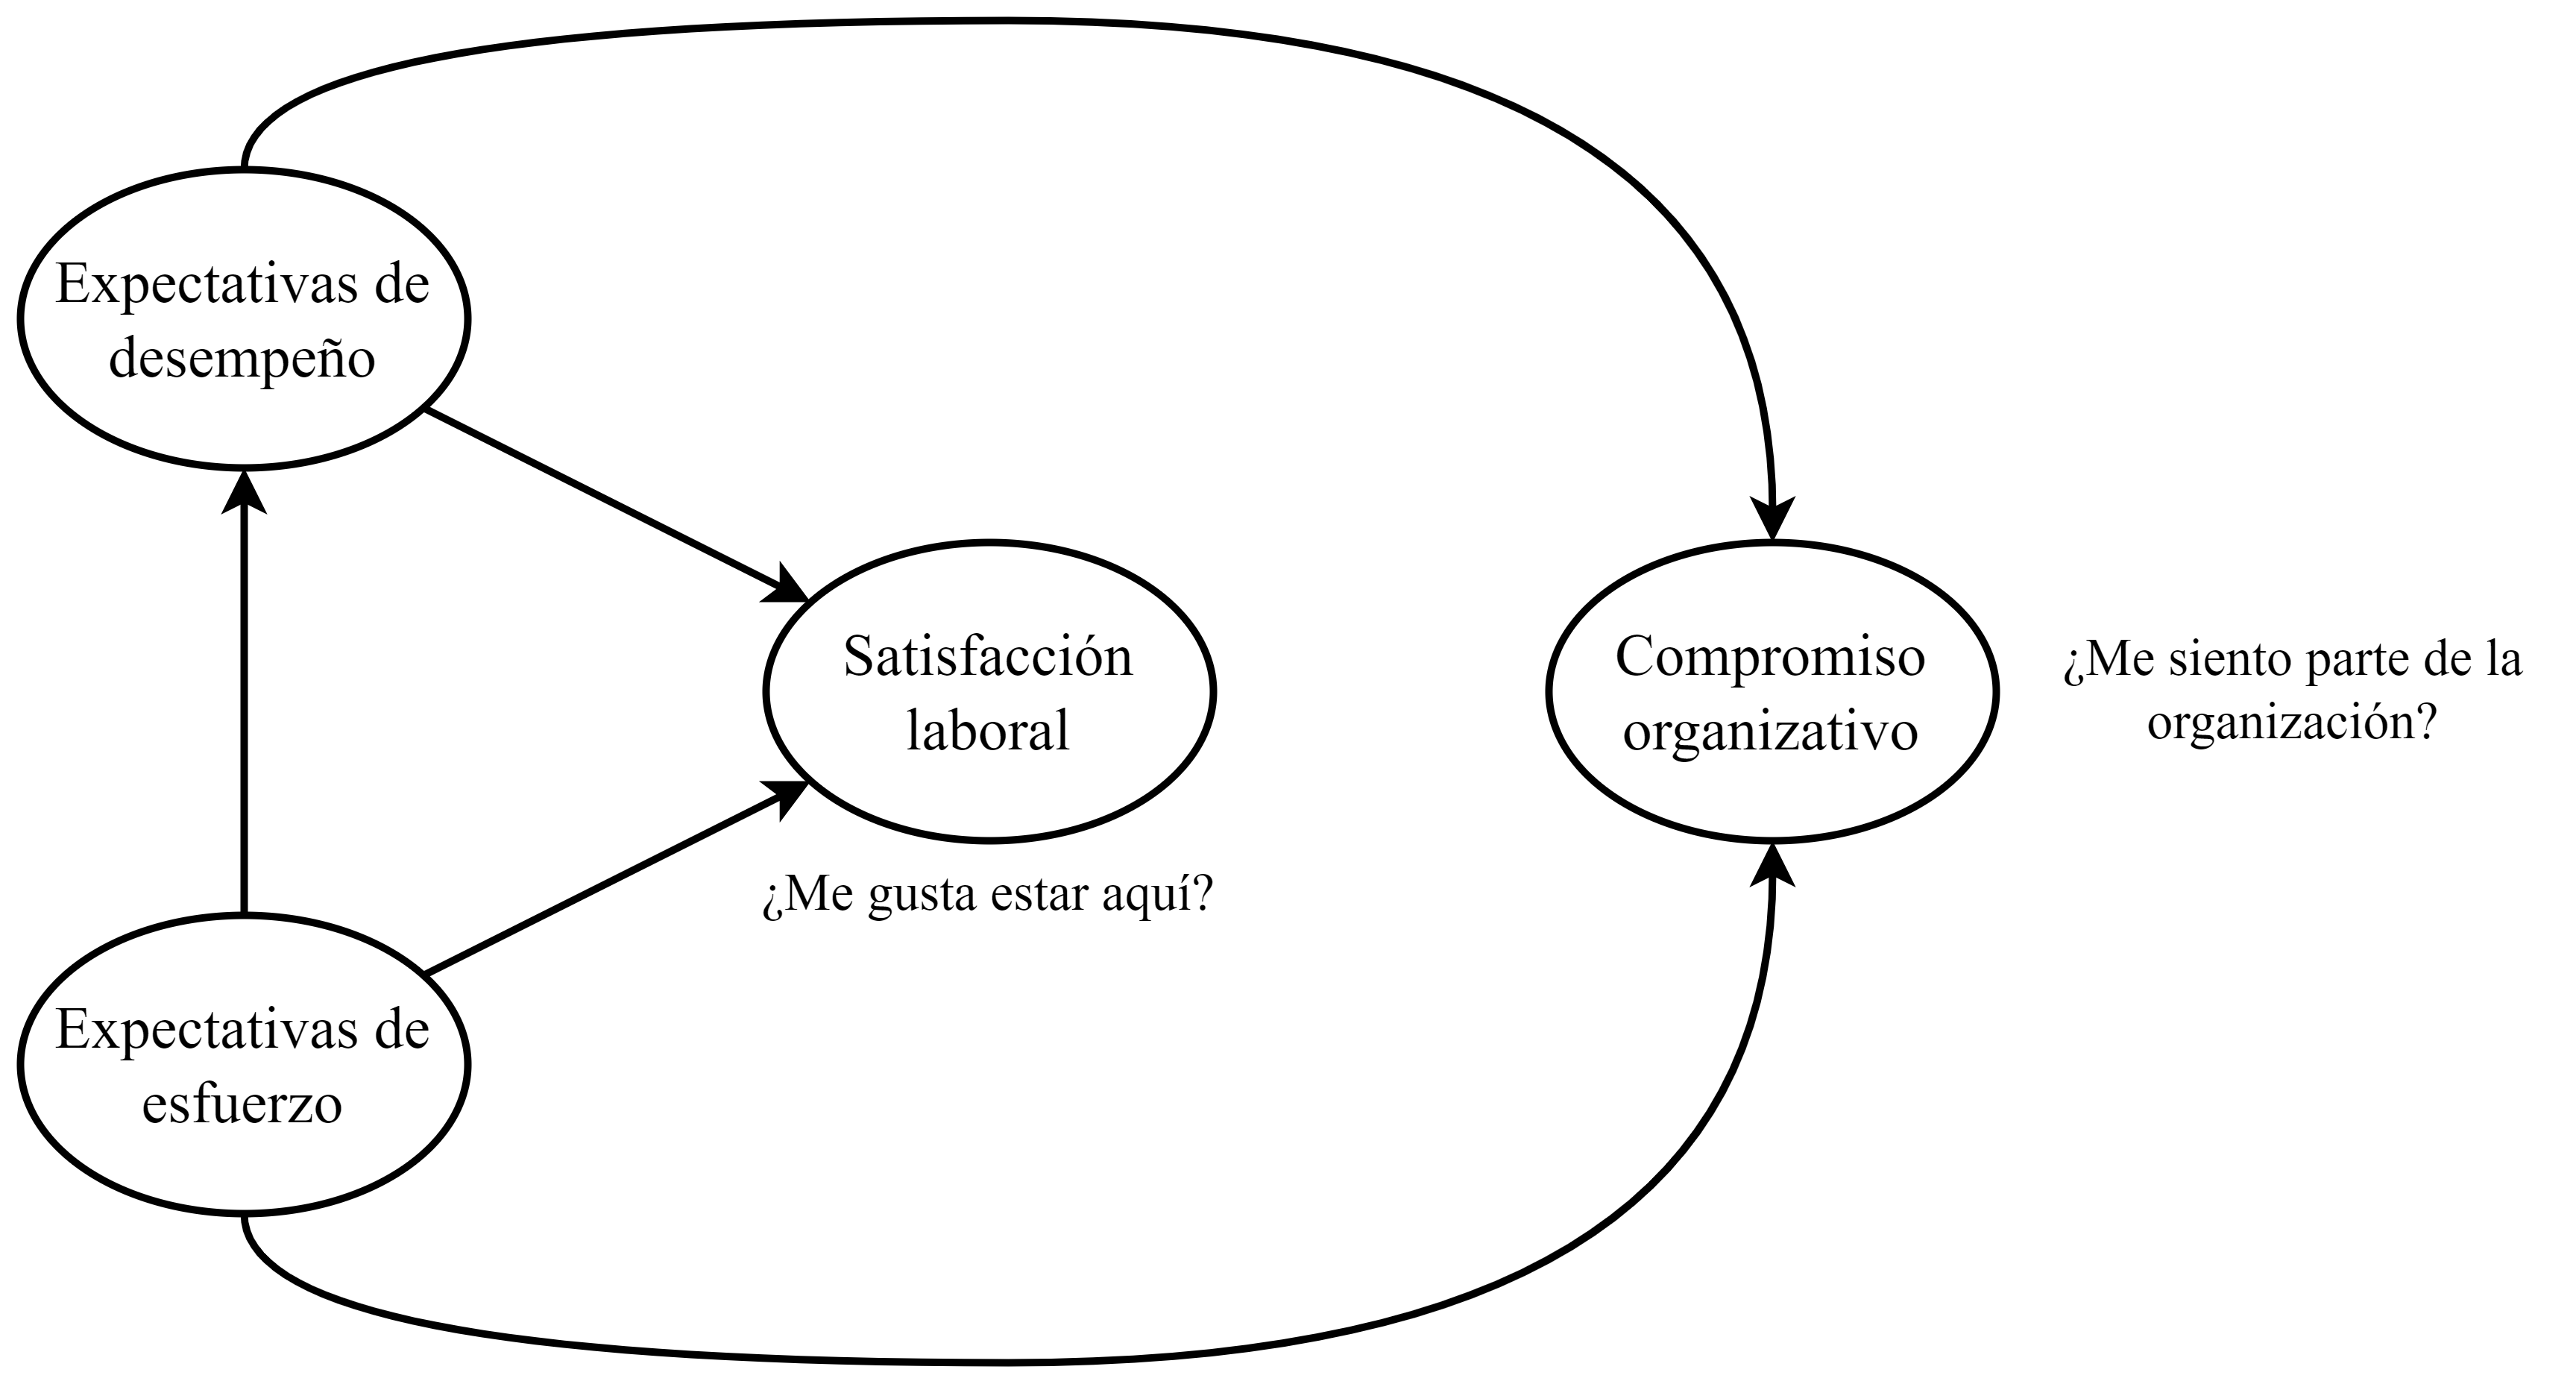
\includegraphics[width=0.5\textwidth]{diagram/Alternativas1.png}
\end{center}
\begin{itemize}
    \item \textbf{Expectativas de desempe\~no:} Si su desempe\~no puede mejorar, su perspectiva del S.I. ser\'a mejor expectativa de desempe\~no alto.
    \item \textbf{Expectativas de esfuerzo:}
    \begin{itemize}
        \item Ante un mayor esfuerzo, la perspectiva del S.I. ser\'a peor, expectativa de esfuerzo bajo.
        \item Ante un menor esfuerzo, la perspectiva del S.I. ser\'a mejor, expectativa de esfuerzo alto.
    \end{itemize} 
\end{itemize}
\subsection{Alternativa de desarrollo del S.I.}

\noindent Basándose en la identificación de fuentes internas o externas existen otras alternativas para el desarrollo de sistemas de información
\begin{center}
    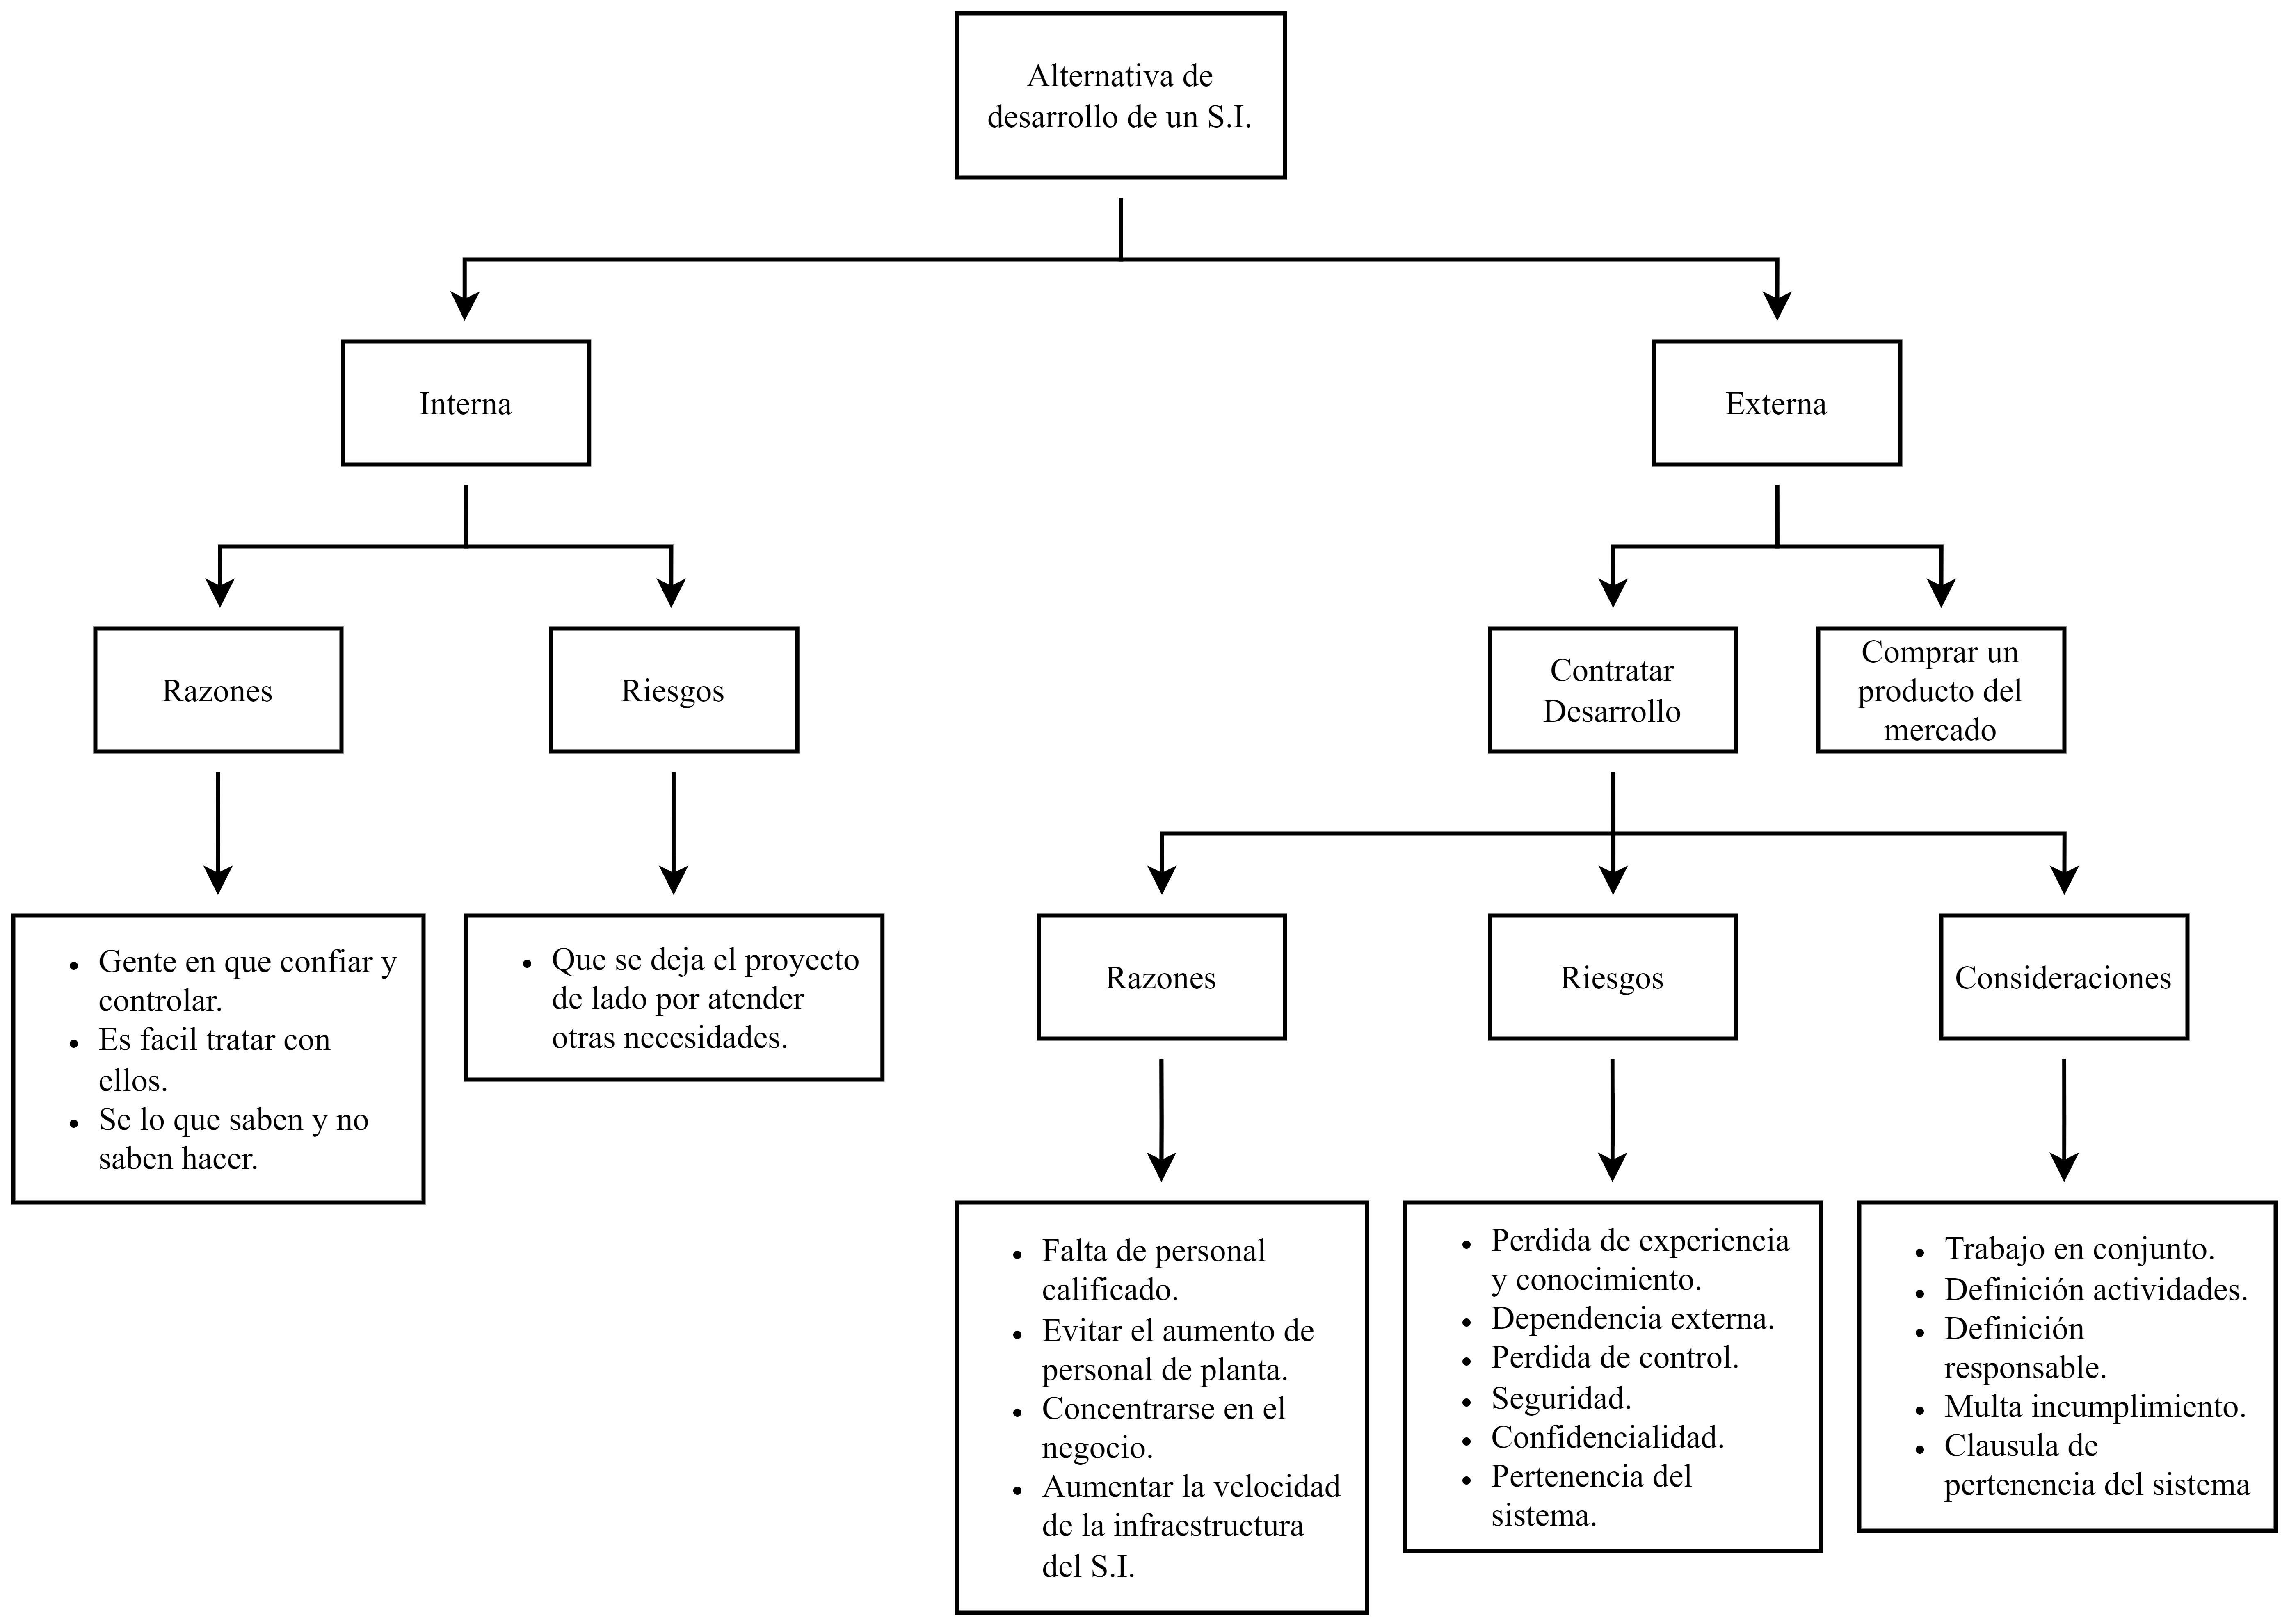
\includegraphics[width=\textwidth]{diagram/Alternativas2.png}
\end{center}

\begin{itemize}
    \item Internas: Fuentes de desarrollo provenientes del mismo entorno empresarial. Pueden ser:
    \begin{itemize}
        \item Agentes internos: Personal perteneciente a la empresa que desarrolla el sistema. Ventajas de recurrir a agentes internos:
        \begin{itemize}
            \item Tienen conocimiento del funcionamiento de la empresa.
            \item La comunicación con estos agentes es mas simple y fluida en comparación con agentes externos.
        \end{itemize}
    \end{itemize}
    \item Externas: Fuentes de desarrollo provenientes de un entorno empresarial diferente. Pueden ser:
    \begin{itemize}
        \item Agentes externos: Personal no perteneciente a la empresa que desarrolla el sistema. Ventajas de recurrir a agentes externos:
        \begin{itemize}
            \item Tienen experiencia en el desarrollo de sistemas de información.
            \item Pueden aportar nuevas ideas y perspectivas al desarrollo del sistema.
        \end{itemize}
    \end{itemize}
    La opciones que ofrece recurrir a fuentes externas de desarrollo son:
    \begin{itemize}
        \item Contratar desarrollo.
        \begin{itemize}
            \item Razones:
            \begin{itemize}
                \item Falta de personal calificado.
                \item Para no tener que aumentar el personal de la empresa.
                \item Se pueden concentrar unicamente en el negocio.
                \item Aumenta la velocidad de desarrollo del SI.
            \end{itemize}
            \item Riesgos:
            \begin{itemize}
                \item Perdida de conocimiento y experiencia una vez los agentes externos terminan el sistema.
                \item Dependencia de los agentes externos en caso de fallas en el sistema.
                \item Perdida del control del desarrollo del sistema.
                \item Seguridad de la información y recursos.
                \item Confidencialidad de la información.
                \item Pertenencia del sistema.
            \end{itemize}
            \item Consideraciones:
            \begin{itemize}
                \item Trabajo conjunto entre agentes internos y externos.
                \item Definición de actividades.
                \item Definición de responsabilidades (funcionalidades y atribuciones).
                \item Multa por incumplimiento.
                \item Clausula de pertenencia del sistema.
            \end{itemize}
        \end{itemize}
        \item Comprar un producto existente en el mercado.
    \end{itemize}
\end{itemize}

\subsection{Restricciones para el desarrollo de un S.I.}
\begin{itemize}
    \item \textbf{Falta de recursos:} No hay Hardware/Softawre, dinero, etc.
    
    \item \textbf{Falta de personal t\'ecnico adecuado:} Inform\'aticos sin experiencia ni conocimientos para construir el S.I.
    
    \item \textbf{Falta de cultura favorable al S.I.:} Resistencia al cambio por parte de los usuarios.
    
    \item \textbf{Falta de claridad de los S.I. necesarios:} No saber qu\'e es lo que se requiere en la empresa.
    
    \item \textbf{Falta de apoyo directivo:} Sin visi\;on sobre los S.I. y/o que estos pueden ayudar al negocio.
    
    \item \textbf{Falta de una visi\'on estrategica de los S.I.} (Engloba todos los puntos anteriores).
\end{itemize}

\section{¿C\'omo cobrar?}
\noindent
Lo que se cobra pero no se dice:
\begin{center}
    \begin{tabular}{|l|c|c|c|}
        \hline
        \textbf{ACTIVIDAD} & \textbf{HH} & \textbf{UF/H} & \textbf{UF total} \\ \hline
        Definici\'on del problema & 10 & M\'as caro : 1 & 10 \\ \hline
        Estudio de factibilidad & 2 & Barato : 0,5 & 1 \\ \hline
        An\'alisis del sistema & 6 & Barato : 0,7 & 4,2 \\ \hline
        Dise\~no l\'ogico & 20 & Caro : 1 & 20 \\ \hline
        Dise\~no f\'isico & 20 & Caro : 0,8 & 16 \\ \hline
        Construcci\'on & 80 & Muy caro : 0,4 & 32 \\ \hline
        Implementaci\'on & 10 & Barato creo : 0,6 & 6 \\ \hline
        \textbf{TOTAL} & & & 89,2 \\ \hline
    \end{tabular}
\end{center}
Lo que si decimos:
\begin{center}
    \begin{tabular}{|l|c|}
        \hline
        \textbf{ACTIVIDAD} & \textbf{UF} \\ \hline
        Estudio sistema & 15,2 \\ \hline
        Dise\~no & 36 \\ \hline
        Programar & 20 \\ \hline
        Probar & 12 \\ \hline
        Capacitar & 4 \\ \hline
        Poner en marcha & 2 \\ \hline
        \textbf{TOTAL} & 89,2 \\ \hline
    \end{tabular}    
\end{center}
Luego se le a\~naden costos extras (dependiendo si es home office o etc) como:
\begin{itemize}
    \item Transporte.
    \item Comida.
    \item Electricidad, agua, internet, etc.
\end{itemize}
Supongamos que son 10 UF de gastos extras, por lo tanto:
\begin{equation*}
    TOTAL = 89,2 \text{ UF} + 10 \text{ UF} = 99,2 \text{ UF}
\end{equation*}

\newpage
\section{Posibles preguntas}
\begin{enumerate}
    \item En el C.V.T.(Ciclo de vida tradicional) ¿Dónde se ve si el sistema hace o no lo que debe?
    \newline
    \textbf{Respuesta:} Se ve casi al final del C.V.T. en la etapa de \hl{Construcción} donde se hacen pruebas para ver si el sistema cumple con los requerimientos.
    
    \item En prototipos y C.V.T. ¿Dónde se necesitan requerimientos tecnológicos?\newline
    \textbf{Respuesta:} En la etapa de \hl{Estudio de factibilidad técnico} se estudia lo necesario, pero se utiliza en \hl{diseño físico} del C.V.T. y en la etapa de \hl{Definición de requerimientos} de los prototipos.

    \item Si observa que el usuario no sabe lo que quiere, ¿Qué estrategia de desarrollo conviene?\newline
    \textbf{Respuesta:} Al no saber lo que quiere el usuario es conveniente usar prototipos. Una estrategia de ciclo de vida tradicional es arriesgada pues ante un cambio de opinion del usuario gran parte del progreso se debera rehacer.

    \item Si tengo una empresa de 'X' cantidad de recursos y puedo asumir 'Y' riesgo, ¿Cuál puesta en marcha usaría y por qué?\newline
    \textbf{Respuesta:} Suponiendo que:
    \begin{itemize}
        \item 'X' es alto y 'Y' es bajo, la mejor opción es la puesta en marcha paralela, pues teniendo varios recursos es mejor tener 2 sistemas funcionando en paralelos ante un posible error del Sistema Nuevo.
        \item 'X' es bajo y 'Y' es alto, la mejor opción es la puesta en marcha inmediata, pues teniendo pocos recursos es mejor tener un sistema en funcionamiento para ahorrar recursos.
        \item Punto medio, la mejor opción es entre puesta en marcha piloto o puesta en marcha gradual, pues ambos son buenas opciones si los recursos y riesgos son indiferentes.
    \end{itemize} 

    \item ¿Cuales son los procesos de desarrollo de un S.I.?\newline
    \textbf{Respuesta:} Concepción, diseño, construcción e implementación.

    \item ¿Qué es la paradoja de la productividad?\newline
    \textbf{Respuesta:} Es cuando se piensa que la implementacion de S.I. y T.I. deben generar mucha productividad, pero realmente al ser un proceso que requiere tiempo, puede hacer parecer que al principio no funciono, pero luego de un tiempo determinado se estabiliza y con el tiempo aumenta la productividad sobrepasando el nivel que habia antes del S.I.

    \item ¿Cuál es la principal razón del fracaso de los S.I.?\newline
    \textbf{Respuesta:} La resistencia al cambio de las personas. Las personas al tener una cultura ya establecida rechazan los S.I.

    \newpage
    \item ¿Cuales son las razones por las que se pueden pedir un S.I.?\newline
    \textbf{Respuesta:} Pueden ser por integrar diversos sistemas en uno solo, para mejorar la velocidad de procesamiento, para mejorar la exactitud y consistencia de sistemas en base numerica, para dar confiabilidad (la gente puede faltar y el conocimiento se va con ellas), para mejorar la seguridad y confidencialidad o para mejorar la imagen de le empresa.

    \item ¿En dónde se conocen los requerimientos?\newline
    \textbf{Respuesta:} Para:
    \begin{itemize}
        \item C.V.T: En la etapa de estudio de factibilidad.
        \item Prototipos: Al principio en la etapa de Requerimientos y luego al final cada vez que se va iterando.
    \end{itemize}

    \item ¿Quién puede pedir un S.I.?\newline
    \textbf{Respuesta:} Lo pueden pedir externos, como gente con poder u organizaciones/estado, o internos, que pueden ser usuarios, especialistas, altos ejecutivos o jefes de departamento.

    \item ¿Qué son los estudios de factibilidad y porque son importantes?\newline
    \textbf{Respuesta:} Nos permite evaluar la fiabilidad del S.I. según los recursos que posee la empresa. Dependiendo de estos estudios se decide si es viable el desarrollo de las demas actividades.

    \item ¿Qué es la reingeniería?\newline
    \textbf{Respuesta:} Es la ingeniería de los procesos. Es una estrategia que cambia o rediseña de manera radical los procesos dentro de la organización con análisis y visión critica. Tiene como objetivo mejorar la eficiencia, calidad y resultados de la organización.

    \item ¿Qué es la industria 4.0?, ¿Cuales son sus aciertos y riesgos?\newline
    \textbf{Respuesta:} La industria 4.0 es una nueva revolución que usa principalmente el internet conbinando técnicas de producción con tecnologías inteligentes. Necesita sistemas para ser monitoreada. Ayuda a mejorar la seguridad de los trabajadores además de que mejora la confiabilidad y velocidad de la empresa. En riesgos es más probable que aumenten los despidos.

    \item ¿Qué es la transformación digital?\newline
    \textbf{Respuesta:} Es la implementación de sistemas digitales en una organización con el fin de automatizar procesos, mejorar su eficiencia y ahorrar costos y tiempos. (Pasar procesos a digital). Mejora a traves del uso de S.I. y T.I.

    \item ¿Qué son las IoT?, ¿Cuál es su importancia?\newline
    \textbf{Respuesta:} Cosas conectadas al internet para hacerlas inteligentes. Su importancia está en un gran uso de tecnologias en las casa ya sea refrigeradores, aspiradoras, etc.
\end{enumerate}

\newpage
\subsection{Contenido Test 2 2022}
Proceso de desarrollo de S.I.:
\begin{itemize}
    \item Concepto de proceso de desarrollo.\newline
    \textbf{Respuesta:} Conjunto de estrategias y t\'acticas planificadas de una empresa. Este se compone por el talento humano de una organizaci\'on y se acompa\~na de herramientas y pr\'acticas para alinear los objetivos de la empresa con los de los colaboradores y as\'i aumentar su compromiso y productividad.
    
    \item Estrategias de desarrollo de S.I.\newline
    \textbf{Respuesta 1:} Es un t\'ermino que engloba todas las acciones y m\'etodos que se utilizan cuando se introducen en el mercado nuevos productos o se modifican los existentes con el objetivo de mejorar los actuales y obtener mayor rentabilida y mejorar los beneficios.
    
    \textbf{Respuesta 2:} La estrategia de S.I. tiene que ver con los usos que hacen las empresas de la tecnolog\'ia para aumentar su valor y mejorar su posici\'on competitiva.
    \begin{itemize}
        \item C.V.T.
        \item Prototipos.
    \end{itemize}
    
    \item Alternativas de desarrollo de S.I.\newline
    \textbf{Respuesta: }
    
    \item Restricciones para el desarrollo de S.I.\newline
    \textbf{Respuesta:}
    \begin{itemize}
        \item Falta de recursos.
        \item Falta de personal t\'ecnico adecuado.
        \item Falta de cultura favorable al S.I.
        \item Falta de claridad de los S.I. necesarios.
        \item Falta de apoyo directivo.
        \item Falta de una visi\'on estrategica de los S.I.
    \end{itemize}
\end{itemize}

\newpage
\subsection{Otras posibles preguntas}
\begin{enumerate}
    \item Los objetivos del S.I.\newline
    \textbf{Respuesta:} Establecer correctamente los objetivos es crucial en el desarrollo de un S.I., ya que implica establecer correctamente las bases, y como las etapas de desarrollo dependen de la etapa anterior, si los objetivos no est\'an correctamente definidos nuestro S.I. no nos servir\'a.

    \item Establecer los l\'imites.\newline
    \textbf{Respuesta:} Definir los l\'imites nos permite diferenciar al sistema de su entorno, y con ello identificar correctamente las salidas y entradas. Esto implica que se usar\'a solo la informaci\'on necesaria y se evitar\'a un aumento de alcance innecesario.

    \item Estudio de factibilidad.\newline
    \textbf{Respuesta:} El estudio de factibilidad nos permite evaluar la fiabilidad del S.I. en funci\'on de los recursos de los cuales disponemos. Este estudio se divide en tres partesL:
    \begin{itemize}
        \item Factibilidad Econ\'omica: Se estudian los beneficios en funci\'on de los costos.
        \item Factibilidad T\'ecnica: Se verifica que se puedan cubrir los requerimientos t\'ecnicos del sistema, tales como tecnolog\'ias y habilidades necesarias.
        \item Factibilidad Operativa: Se verifica que el sistema se pueda implementar sin afectar negativamente a los procesos y operaciones ya existentes.
    \end{itemize}
\end{enumerate}
% \subsection{Test 2 2024}
% (En las palabras que recuerdo) Explique porque es importante efectuar:
% \begin{itemize}
%     \item La definici\'on del problema.
%     \item Capacitaci\'on.
%     \item 
% \end{itemize}
\end{document}